\documentclass[a4paper, 11pt]{article}
\usepackage[utf8]{inputenc}
\usepackage[left=1in,right=1in,bottom=0.8in]{geometry}
\usepackage{enumitem}
\usepackage{graphicx}
\graphicspath{ {Figures/} }
\usepackage{float}
\usepackage[labelfont=bf]{caption}
\usepackage{fixltx2e}
\usepackage{caption}
\usepackage{amsmath}
\usepackage{capt-of}
\usepackage{tabu}
\let\svthefootnote\thefootnote

\title{\bf Experiment 1\\ Characterization of a CMOS Inverter}
\author{\it Dhruv Ilesh Shah | 150070016}
\date{January 6, 2017}


\begin{document}
\maketitle
\section{Overview}
The CMOS inverter is one the simplest CMOS logic gate, and an essential component of all digital circuits. In this experiment, we characterize the CMOS inverter and observe its DC \& AC behaviour. In particular, we observe the following.
\begin{itemize}[label= $\rightarrow$]
	\item DC Transfer Characteristics
	\item Output Characteristics
	\item Delay Characteristics
	\item Delay variation with supply voltage
	\item Current drawn by the Ring Oscillator
\end{itemize}
For transfer and output characteristics, IC \emph{MM74C04} was used. The delay measurements and variations for a single CMOS inverter require very accurate instruments and hence, for the delay measurement tasks, a ring oscillator with {\it17} inverters was used. Variation of the period of oscillation with the load can be used to obtain a good estimate on the delay. The superposition of the switching currents of all the inverters is observed in the last part, as the total current drawn from the power source.
\par In Section 2 of this report, I present a brief overview of the experimental setup for the various sub-parts of the experiment performed. This is followed by the observations from the experiments, with figures of the waveforms wherever relevant. The answers to the assignment questions are also present.

\section{Observations}
Each part of the experiment essentially involves the CMOS inverter as the elementary unit. For this, I have used the IC \emph{MM74C04} provided. The Opamp buffer ({\em TL072}) was introduced so that the DSO does not add extra load to the circuit during the act of measurement. Circuit layouts for the various parts of the experiment are shown below.
\vspace{1em} \\
{\bf Components Used: }MM74C04 $\times 4$, TL072, Decoupling Capacitors (0.1$\mu$F) $\times 2$, 20 K$\Omega$ potentiometer, resistors (1.2K$\Omega$, 1$\Omega$).
\newpage
\subsection{DC Transfer Characteristics}

The most important characteristic of the CMOS inverter is the switching voltage $V_{sw}$. To find this, we must plot the transfer characteristics of the device. The circuit layout is as given below.

\begin{figure}[h]
\centering
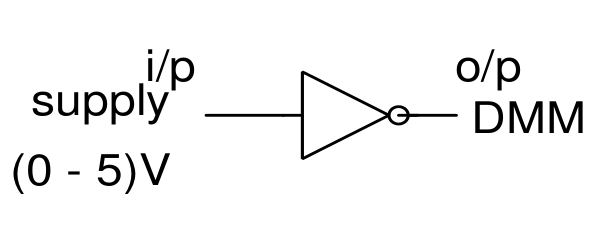
\includegraphics[scale=0.3]{fig1}
\caption{Observing the DC Transfer Characteristics}
\end{figure}

\hspace*{-2em} As we increase the input voltage from 0 to $V_{DD}$, the output is expected to fall from $V_{DD}$ to 0.

\begin{center}
\begin{tabular}{| c | c |}
\hline
{\bf V\textsubscript{in}} & {\bf V\textsubscript{out}}\\
\hline
0.3 & 5.01 \\1.3 & 5 \\1.4 & 4.99 \\1.6 & 4.96 \\1.7 & 4.91 \\1.9 & 4.8 \\2 & 4.64 \\2.1 & 4.53 \\2.19 & 4.28 \\2.2 & 4.08 \\2.215$^*$ & 3.43 \\2.23$^*$ & 2.16 \\2.245$^*$ & 1.81 \\2.26$^*$ & 1.34 \\2.275$^*$ & 0.65 \\2.29 & 0.51 \\2.3 & 0.36 \\2.4 & 0.24 \\2.5 & 0.14 \\2.6 & 0.11 \\2.7 & 0.07 \\2.8 & 0.05 \\2.9 & 0.035 \\3 & 0.02 \\3.1 & 0.009 \\3.2 & 0.0036 \\3.5 & 0.0001 \\
\hline
\end{tabular}
\captionof{table}{DC Transfer Characteristics of the given CMOS inverter}
\end{center}
The readings suggest a near ideal behaviour of the inverted with the $V_sw \approx 2.2V$. The behaviour can be better represented by plotting V\textsubscript{out} versus V\textsubscript{in} as shown in figure 2.
\let\thefootnote\relax\footnotetext{\hspace{-2em}$^*$Considering the least count of the Voltmeter, readings between 2.2V and 2.3V could not be obtained precisely, but the fall in $V_{out}$ is very steep, and hence the interpolation was done. The values of $V_{out}$ were not manipulated.}

\begin{figure}[H]
\centering
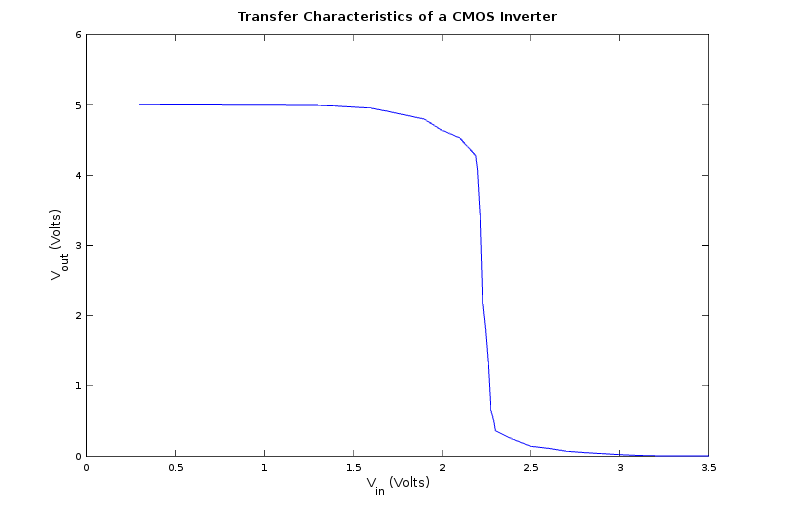
\includegraphics[scale=0.55]{Transfer_Characteristics}
\caption{}
\end{figure}
But we have
$$
V_{sw} = \frac{\sqrt{\beta_p}(V_{DD}-V_t) + \sqrt{\beta_n}V_t}{\sqrt{\beta_p} + \sqrt{\beta_n}}
$$
Substituting the values\addtocounter{footnote}{0}\let\thefootnote\svthefootnote\footnote{\em(Here, I have used $V_t \approx 1V$)} gives $\frac{\beta_p}{\beta_n} \approx \frac{4}{9}$.  
\subsection{Output Characteristics}
The CMOS inverter is used widely in many circuits, and hence it is very important to model the output characteristics of the device. The figures 4 and 5 represent the output characteristics of the device, measure according to the circuit arrangement below.
\begin{figure}[H]
\centering
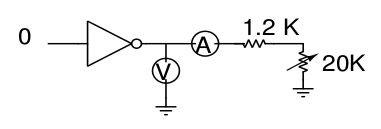
\includegraphics[scale=0.7]{fig2}
\caption{Ciruit Layout for observing output characteristics at {\em low input}}
\end{figure}
\noindent A similar layout was used for measuring the characteristics at high input.\\
The highly linear behaviour, with the change in the variable resistance suggests that the output impedance is largely constant.
\newpage
\begin{figure}[H]
\centering
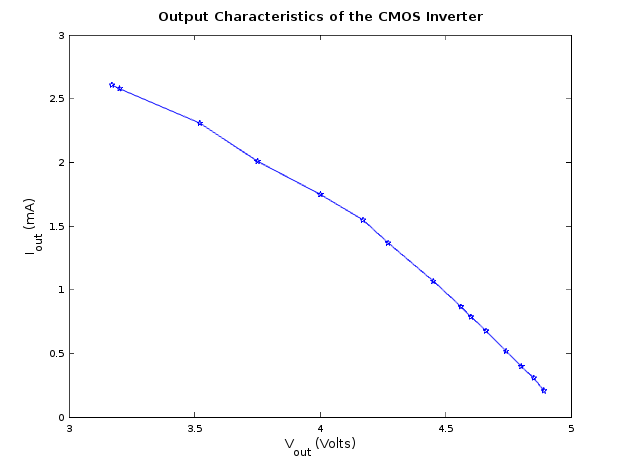
\includegraphics[scale=0.6]{Output_0}
\caption{Output Characteristics with $V_{in} = 0$}
\end{figure}
\begin{figure}[H]
\centering
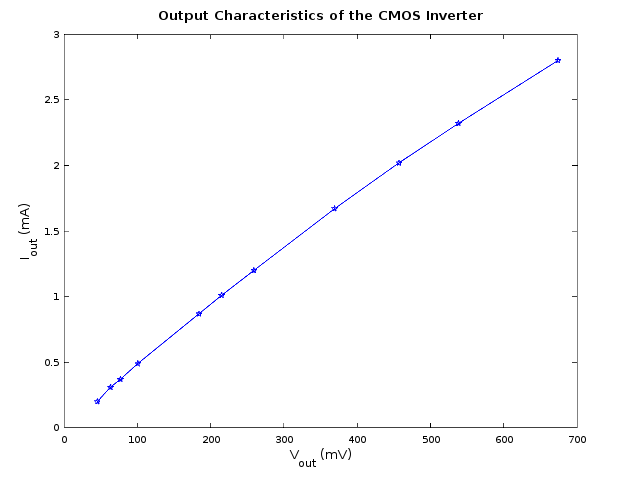
\includegraphics[scale=0.6]{Output_1}
\caption{Output Characteristics with $V_{out} = V_{DD}$}
\end{figure}

\begin{table}[H]
\centering
\begin{tabular}{| c | c |}
\hline
\bf Voltage (Volts) & \bf Current (mA)\\
\hline
4.89 & 0.21 \\4.85 & 0.31 \\4.8 & 0.4 \\4.74 & 0.52 \\4.66 & 0.68 \\4.6 & 0.79 \\4.56 & 0.87 \\4.45 & 1.07 \\4.27 & 1.37 \\4.17 & 1.55 \\4 & 1.75 \\3.75 & 2.01 \\3.52 & 2.31 \\3.2 & 2.58 \\3.17 & 2.61\\
\hline
\end{tabular}
\caption{Output Characteristics with $V_{in} = 0$}
\end{table}

\begin{table}[H]
\centering
\begin{tabular}{| c | c |}
\hline
\bf Voltage (mV) & \bf Current (mA)\\
\hline
45.4 & 0.2 \\63.3 & 0.31 \\76.8 & 0.37 \\100.6 & 0.49 \\184.2 & 0.87 \\215 & 1.01 \\259 & 1.2 \\369 & 1.67 \\457 & 2.02 \\538 & 2.32 \\674 & 2.8 \\
\hline
\end{tabular}
\caption{Output Characteristics with $V_{out} = V_{DD}$}
\end{table}

\subsection{Delay Characterization of the Inverter}
An inevitable feature of an inverter is the delay introduced by it, especially in a digital circuit. This delay however, is very small for each independent inverter module and hence would require highly sophisticated apparatus for monitoring. A workaround is to use a ring oscillator and model the delay indirectly, as performed in this part of the experiment.\par
For this part, a 17-stage ring oscillator was used. We rely on the fact that the delay of an inverter can be modelled as $$
d_{abs} = k_0 + k_1C_{load}
$$ where $C_{load}$ is the load capacitance being driven, which can be controlled by varying the number of load nodes. The basic equations guiding this scenario, in a simplified format are as follows.
\begin{equation*}
\begin{split}
d_{abs} &= k_0 + \tau_{inv}\frac{C_{load}}{C_{in}} \\
d_{inv} &= p_{inv} + \frac{C_{load}}{C_{in}}
\end{split}
\end{equation*}
\vspace*{3.5em}
\begin{table}[H]
\centering 
  \begin{tabular}{ c  c }
      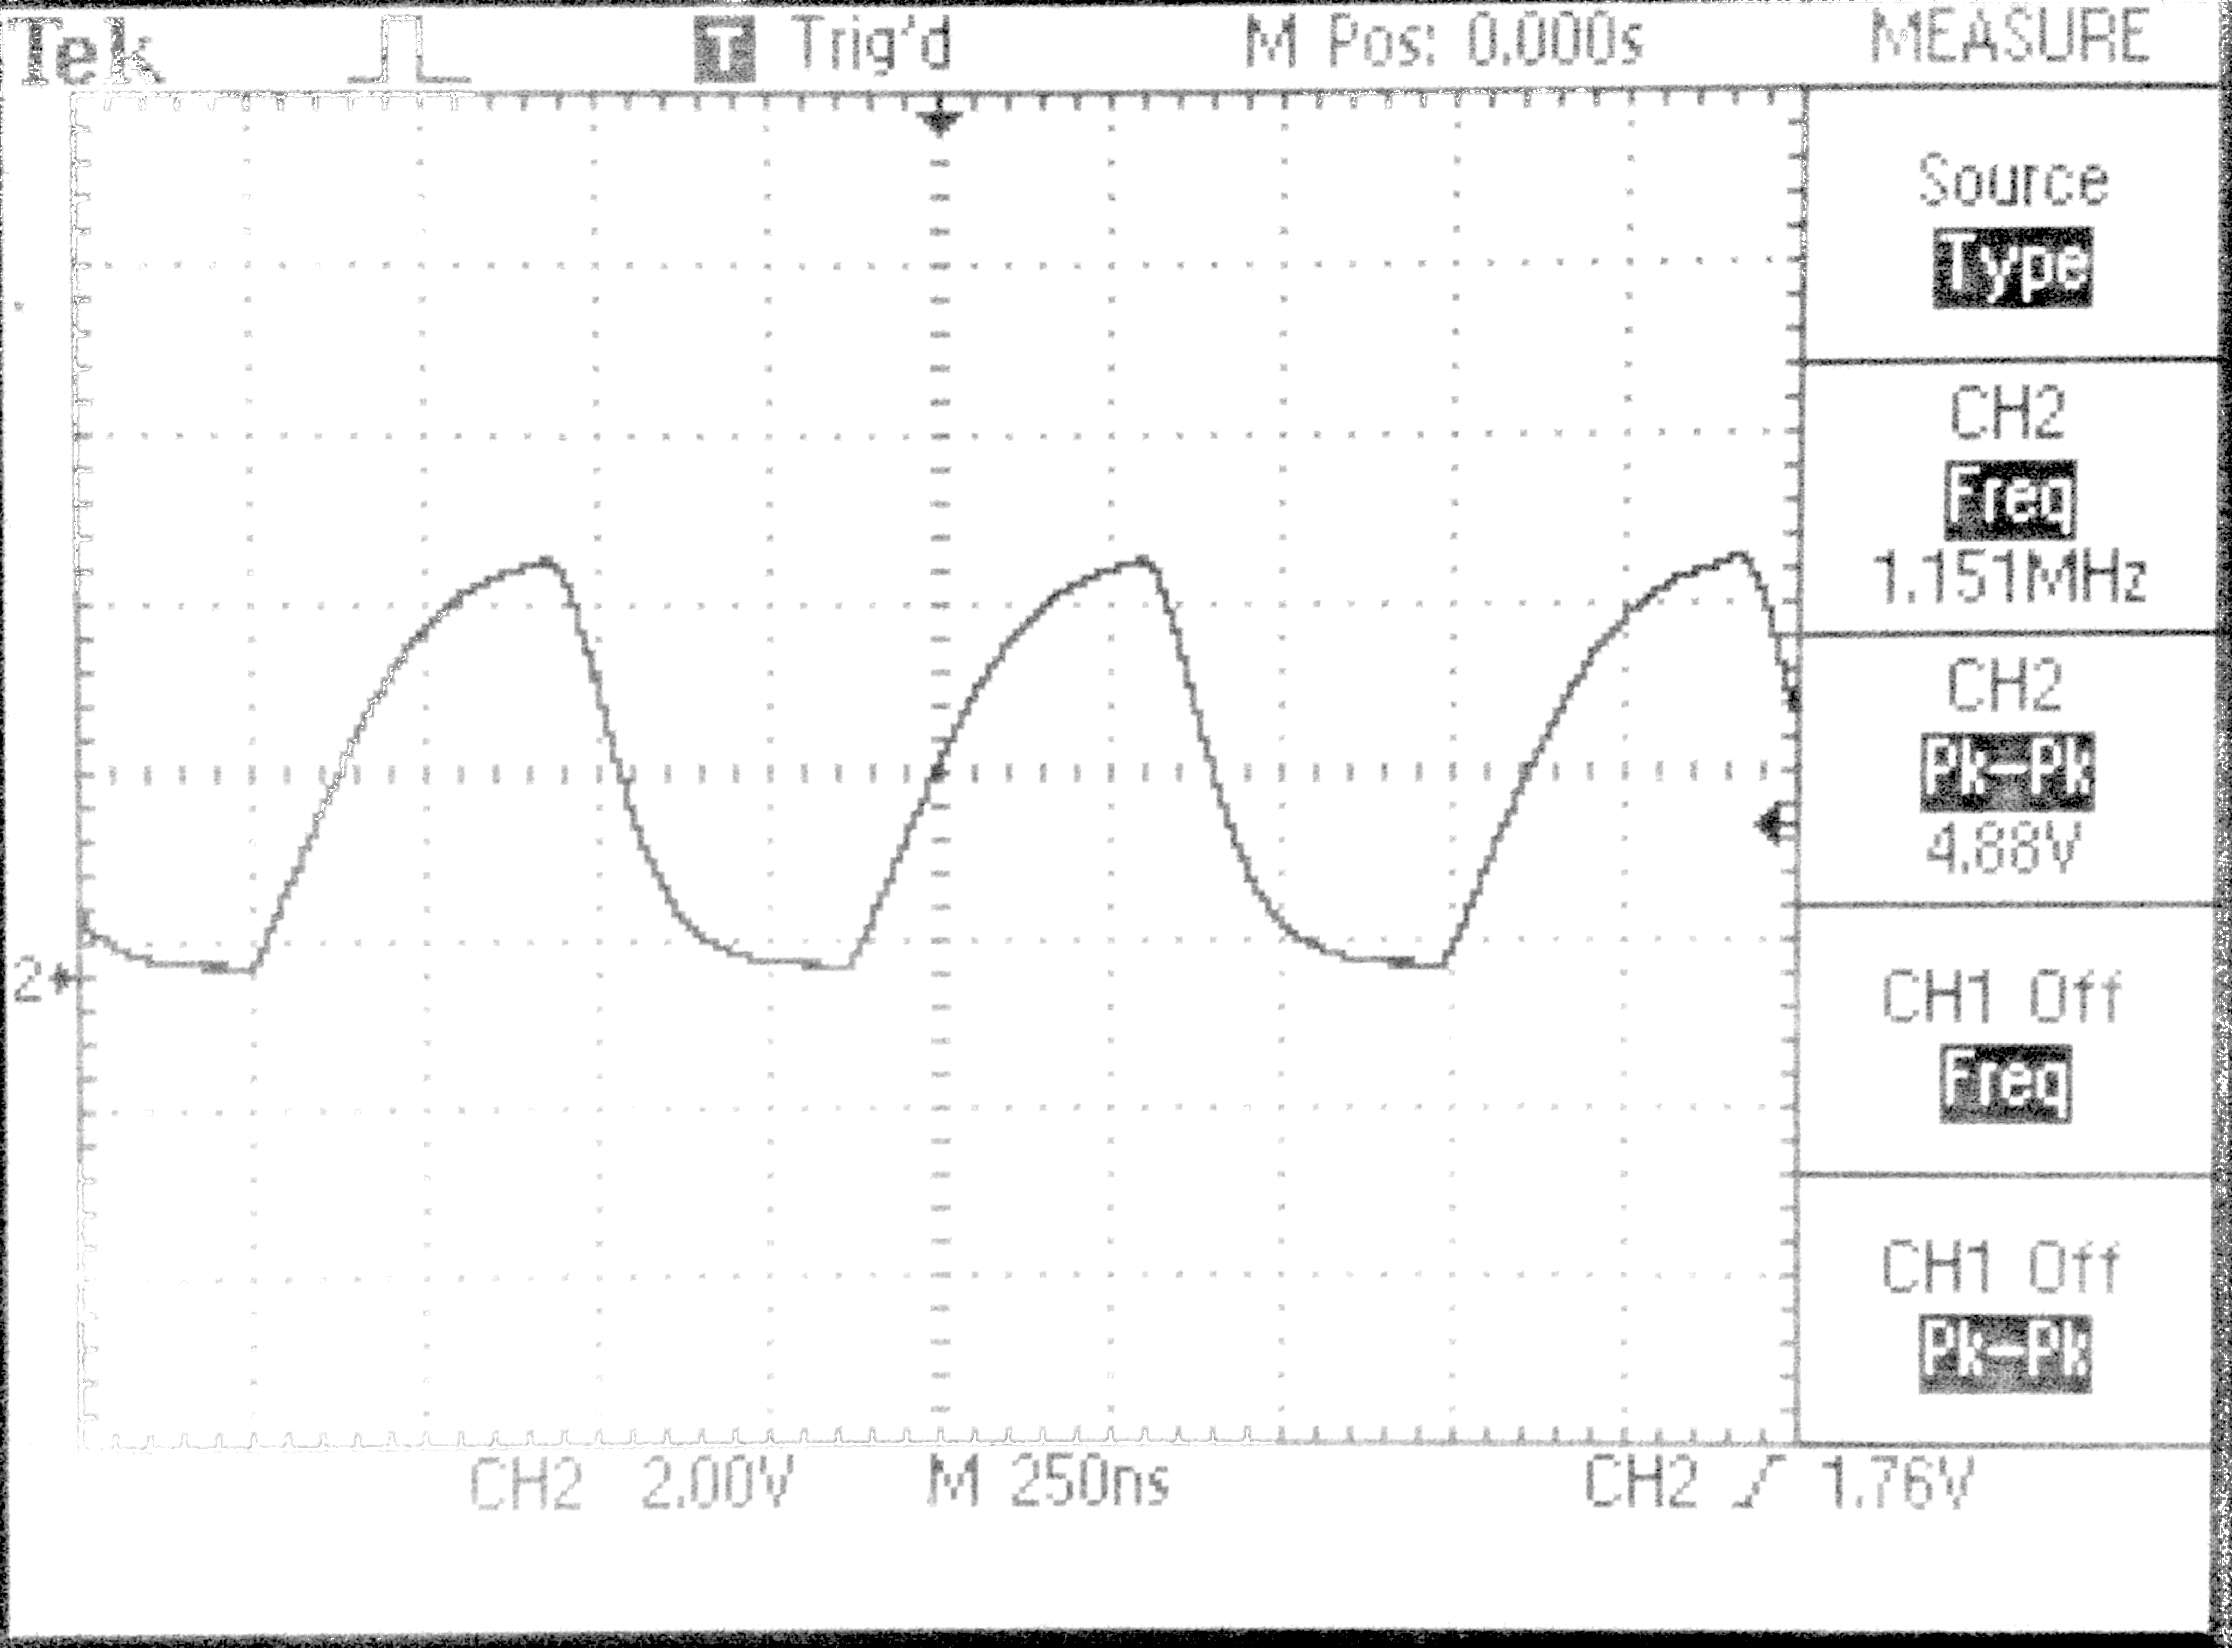
\includegraphics[width=2.5in]{EE214_1.jpg} & 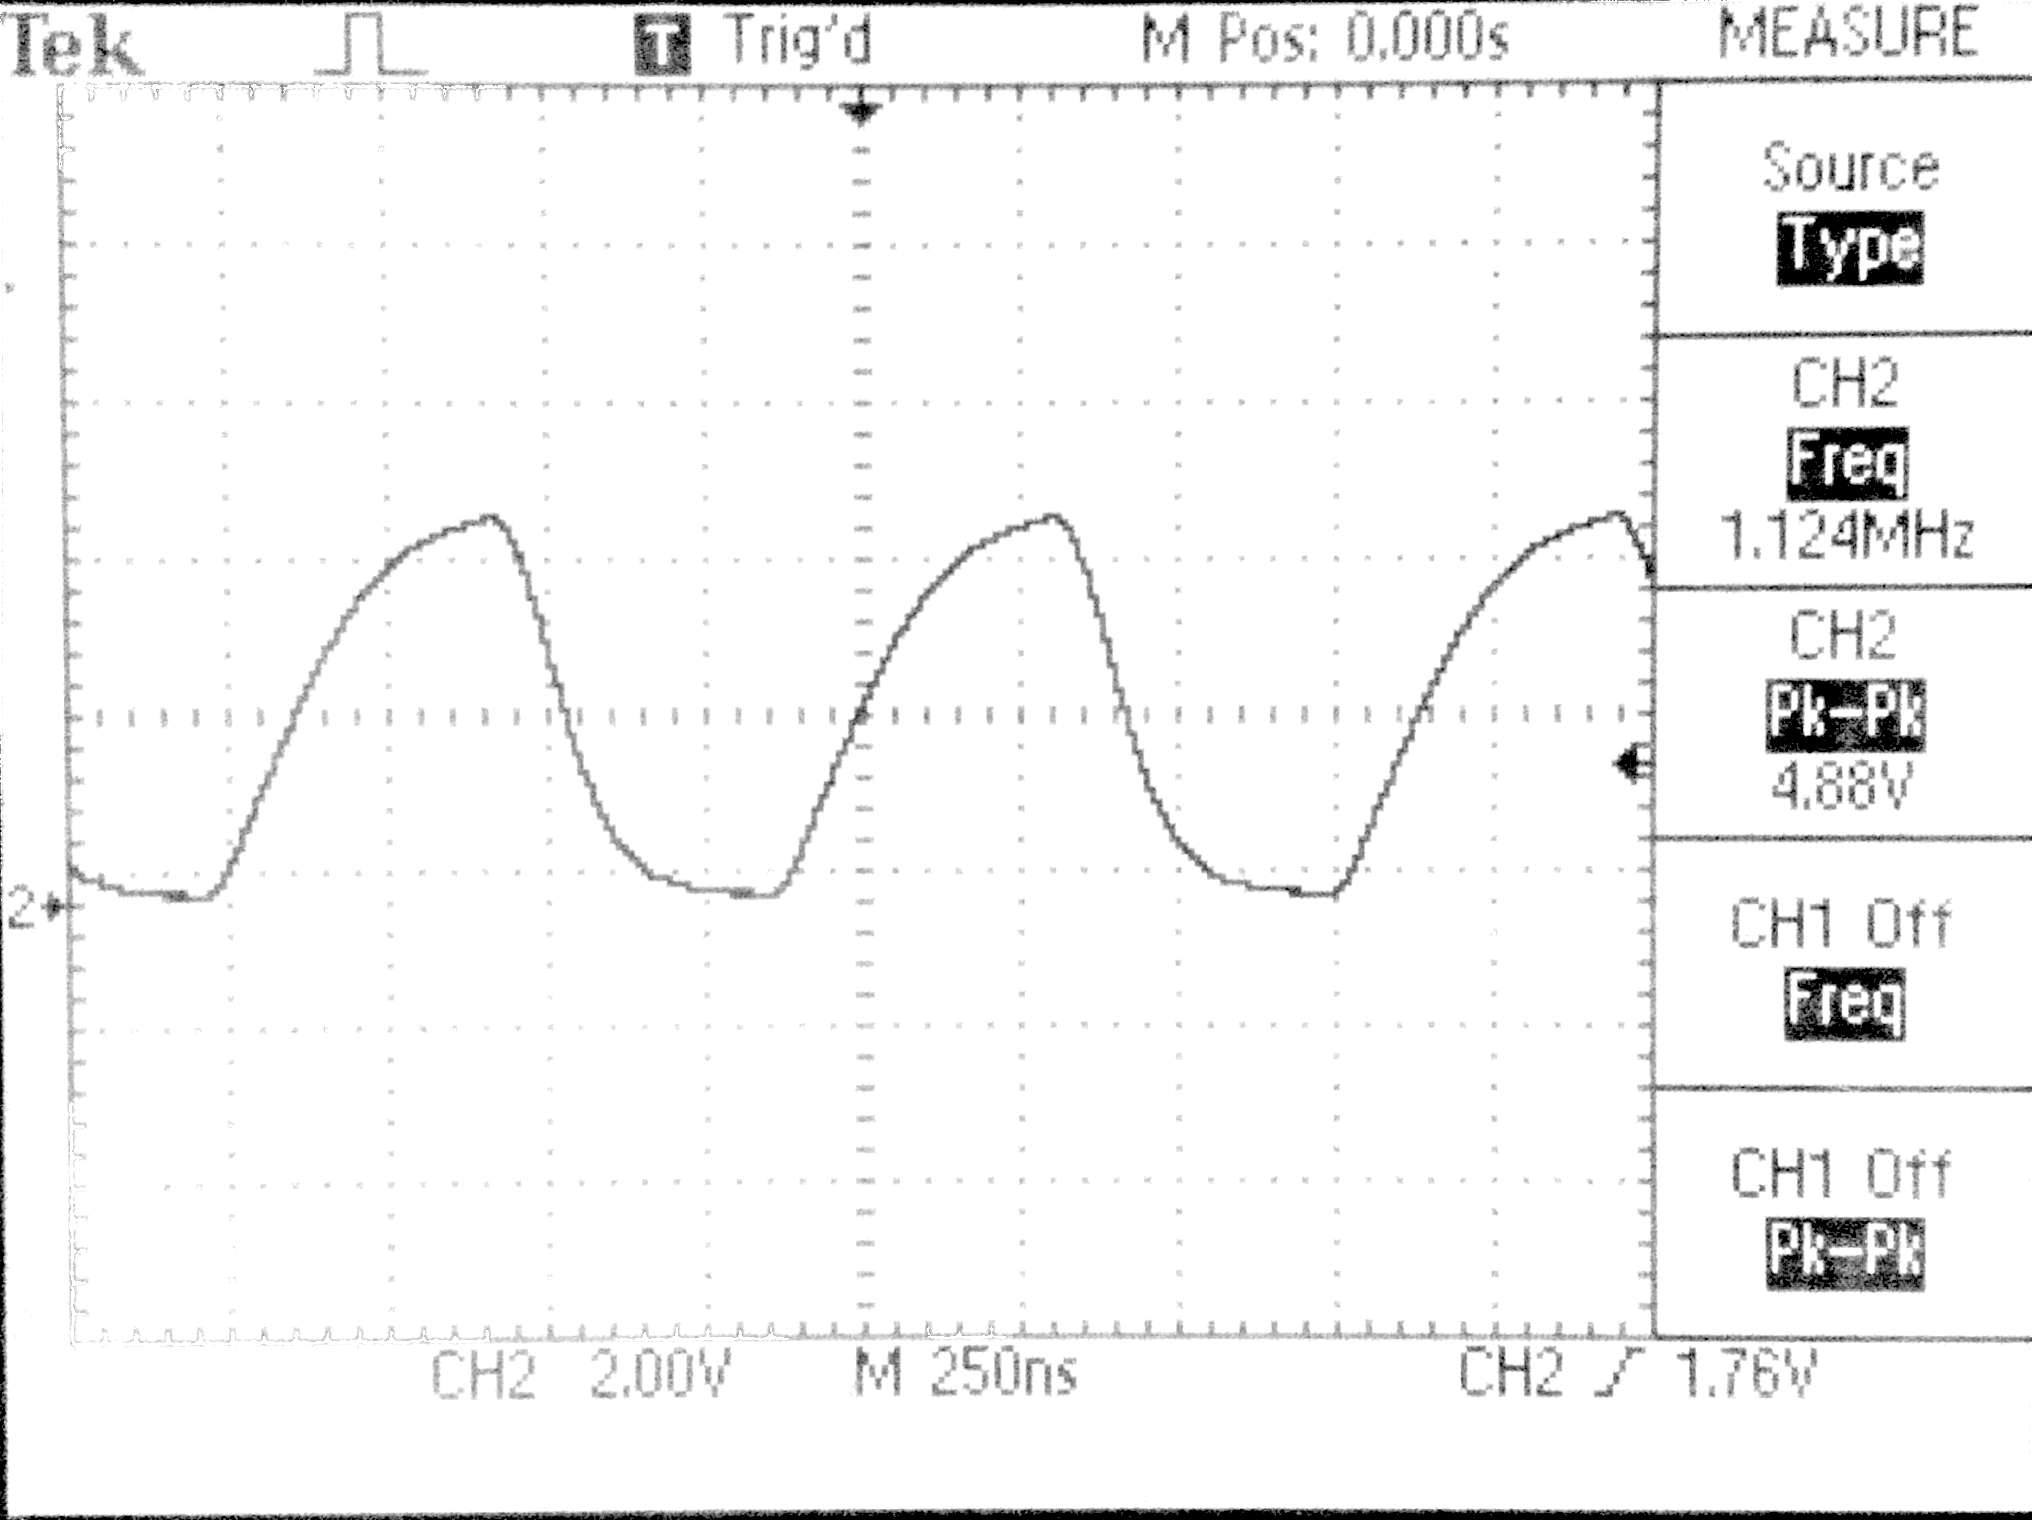
\includegraphics[width=2.5in]{EE214_2.jpg} \\
      \em Load = 2 & \em Load = 3 \\
         & \\
      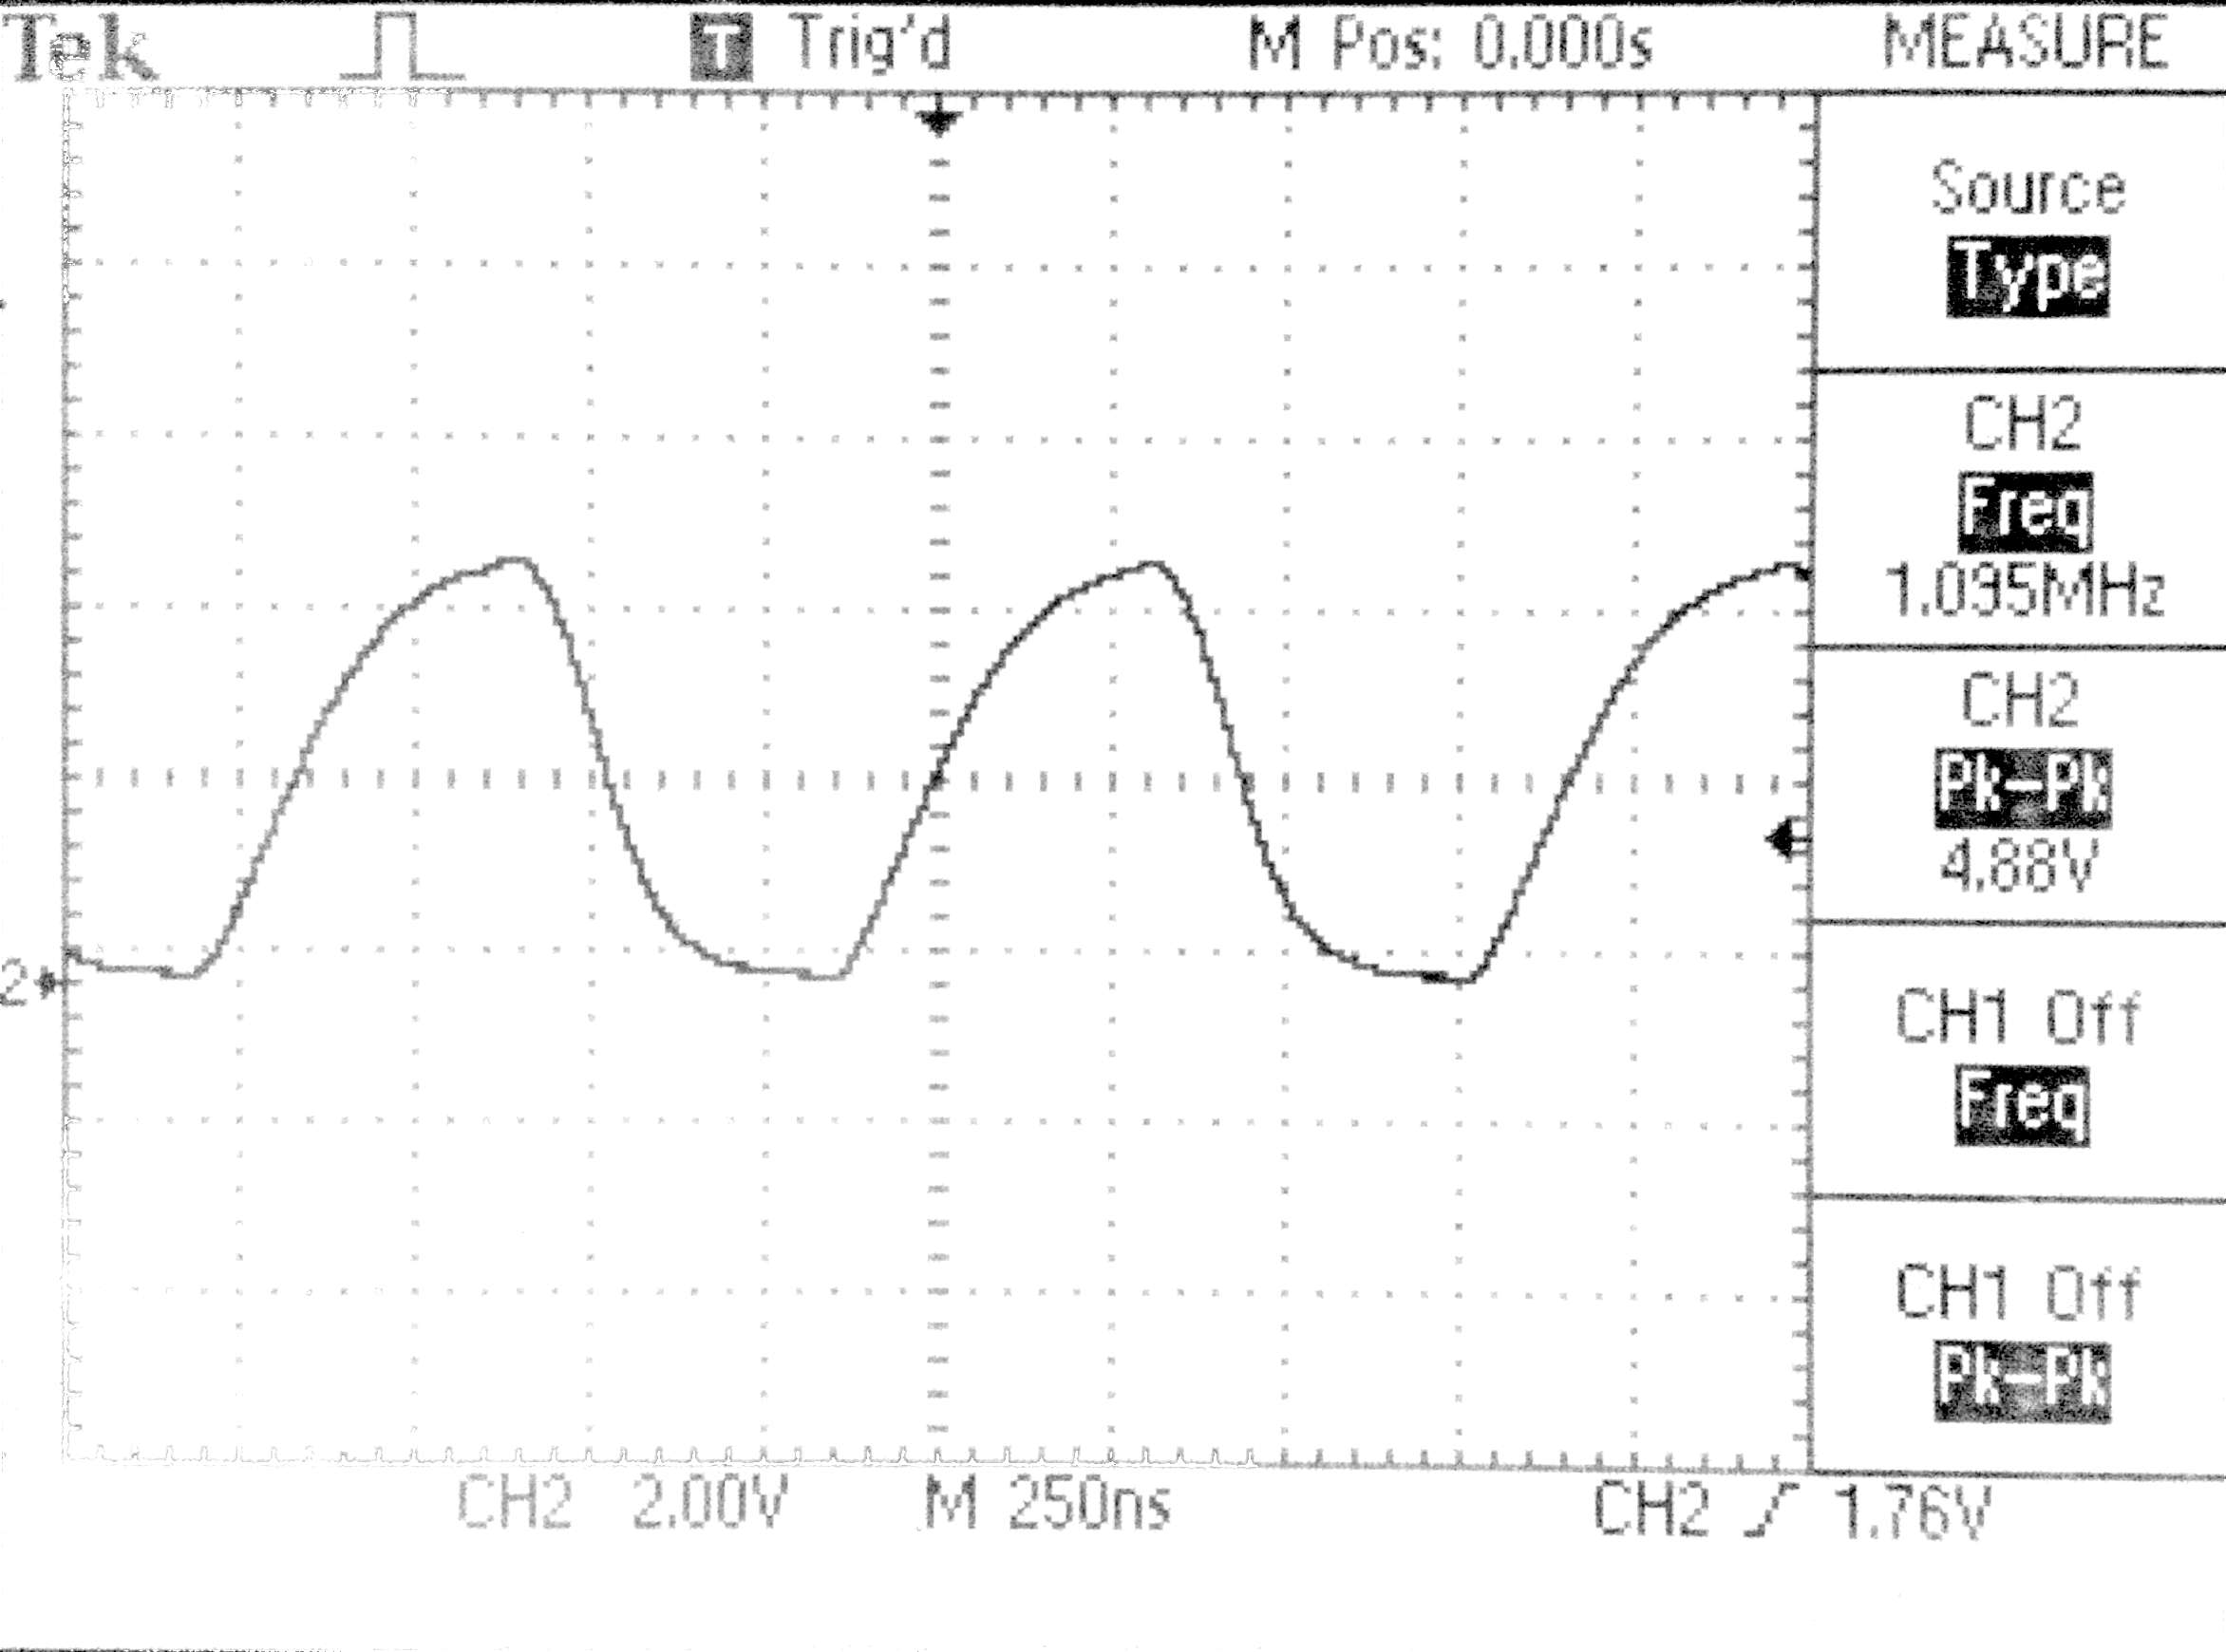
\includegraphics[width=2.5in]{EE214_3.jpg} & 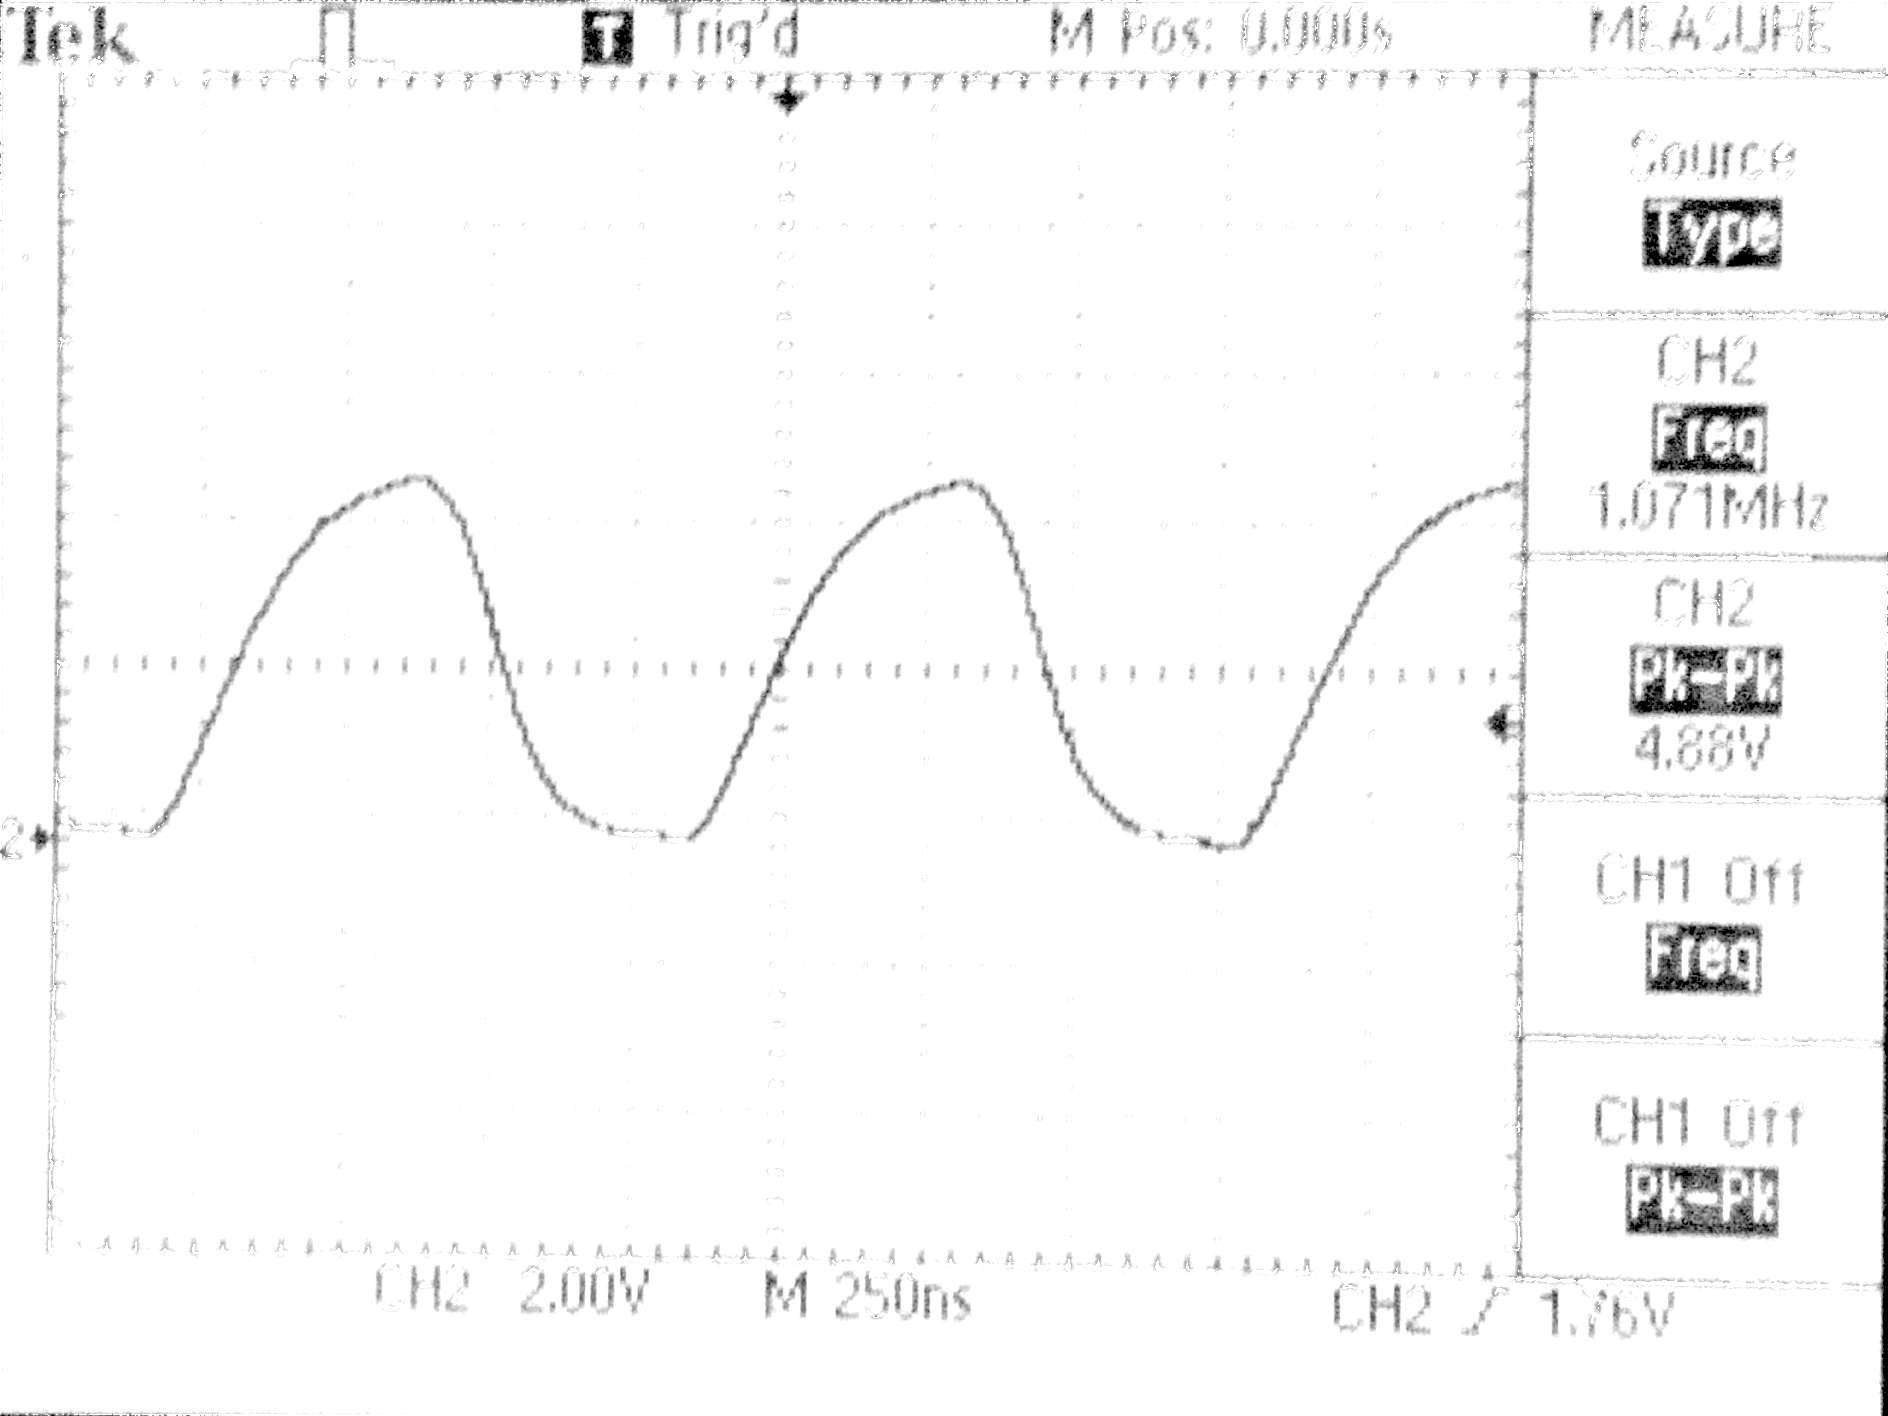
\includegraphics[width=2.5in]{EE214_4.jpg} \\
      \em Load = 4 & \em Load = 5 \\
  \end{tabular}
 \caption{Snapshots of the output waveform at different loads ($V_{DD} = 5V$)}
 
\end{table}

\begin{table}[H]
\centering
\begin{tabular}{| c | c |}
\hline
\bf Number of Load Nodes & \bf Frequency (MHz)\\
\hline
2 & 1.151 \\
3 & 1.124 \\
4 & 1.095 \\
5 & 1.071 \\
\hline
\end{tabular}
\caption{Variation of the frequency of oscillation with load {\em($V_{DD} = 5V$)}}
\end{table}
Clearly, an increase in the load results in a lowering of the frequency and hence an increase in the period of oscillation. The relation is better shown as a plot.\\
\begin{figure}[H]
\centering
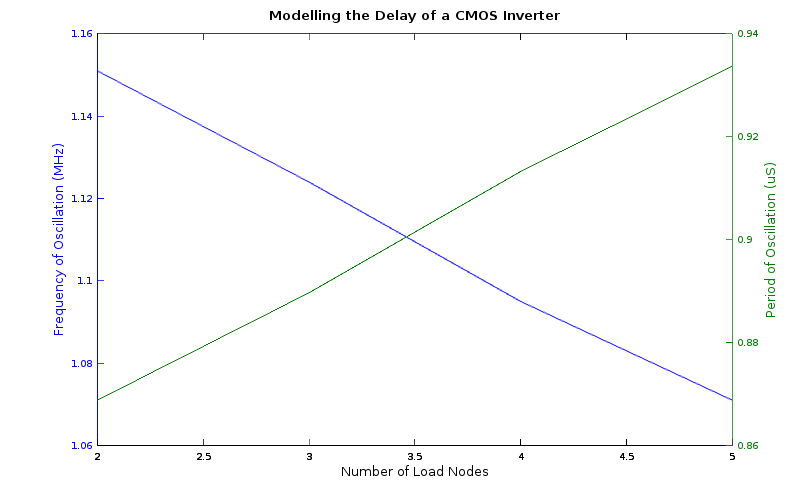
\includegraphics[scale=0.55]{Delay_Char}
\caption{}
\end{figure}
%From the slope of the {\em Period|Load} plot, we get $\tau = 0.133 \mu s$. This gives $p_{inv} = 39.03$.
\vspace*{2em}
We have period of oscillation given by
$$
\tau \times (34p_{inv} + (32 + (2\times (1 + Additional Load Output)))
$$
measured in seconds, given the rise and fall times are equal.
We thus have
\begin{equation*}
\begin{split}
Slope &= 2\tau = 0.022 \mu s \\
Intercept &= 34(\tau (p_{inv} + 1)) = 0.827
\end{split}
\end{equation*}
From above, we have 
\begin{equation*}
\begin{split}
\tau &= 0.011\mu s \\
p_{inv} &= 1.21
\end{split}
\end{equation*}


\subsection{Delay Variation with Supply Voltage}
An essential feature of the CMOS inverter is that we can assume the analog device to be digital, and operational on digital H/L voltages. The definition of this high/low, however, does affect the characteristics and in this part, I have presented the variation of the delay with change in $V_{DD}$. \\
From theory,
$$
Period \propto \frac{V_{DD}}{(V_{DD} - V_t)^2}
$$ In this exercise, I will demonstrate the same relation, from experimental observations.

\begin{table}[H]
\centering 
  \begin{tabular}{ c  c }
      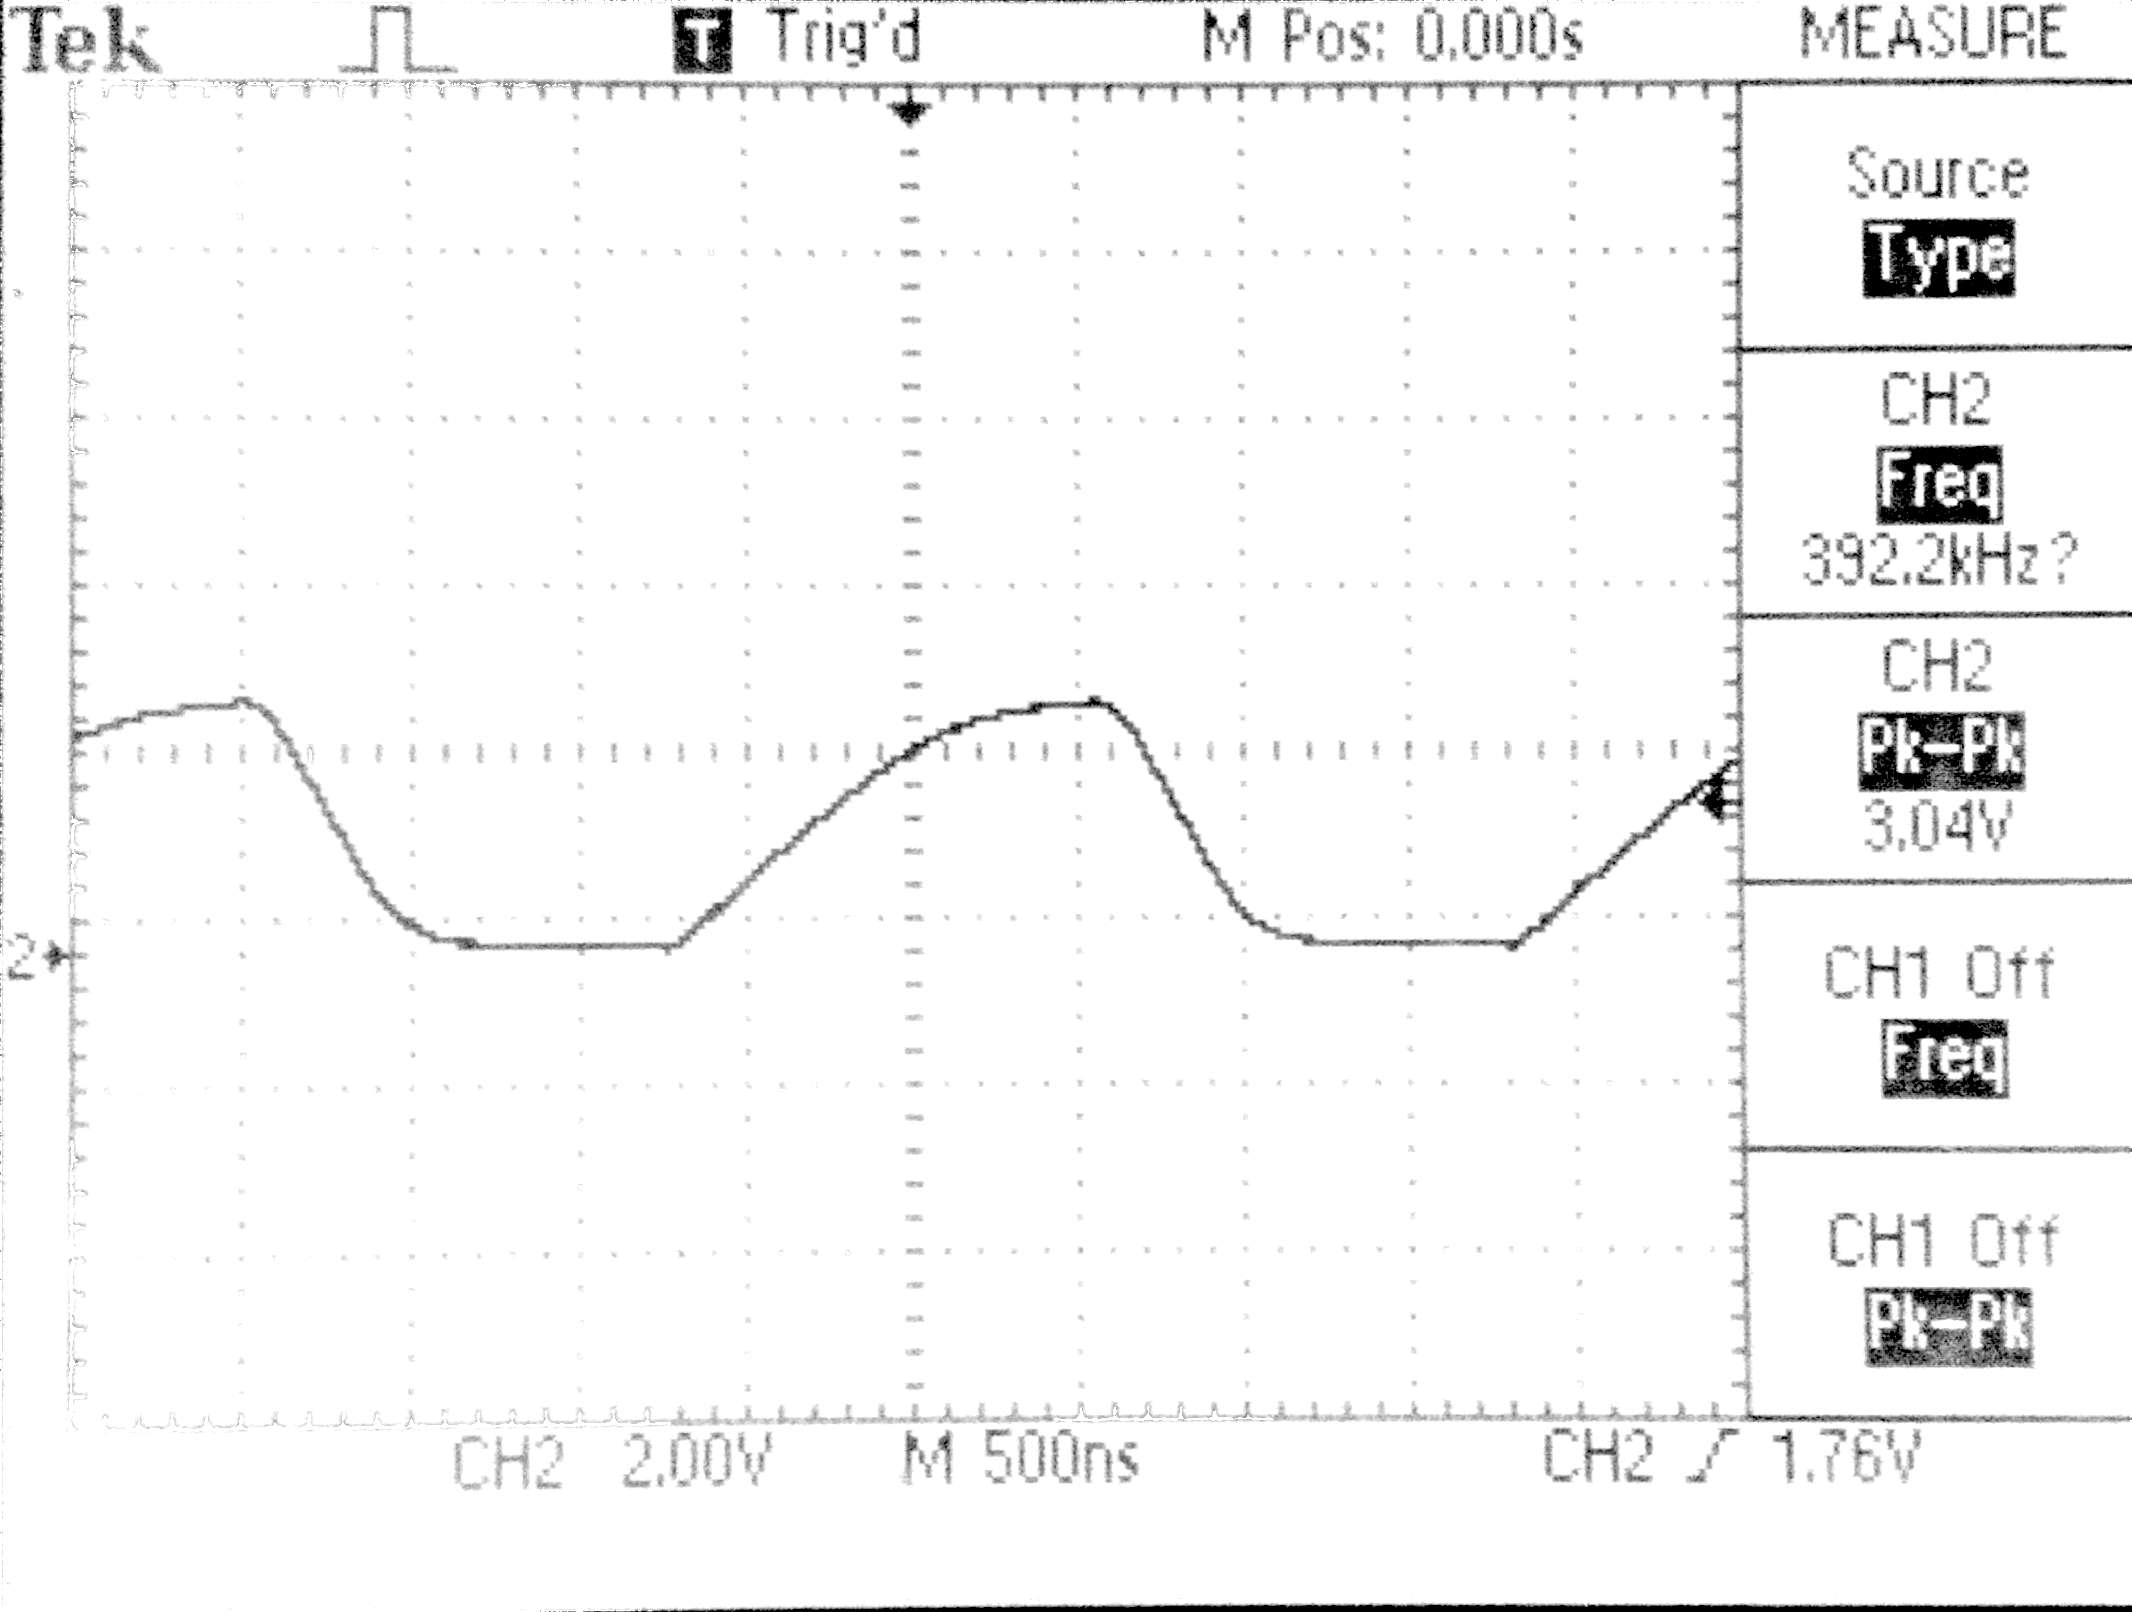
\includegraphics[width=2.5in]{EE214_7.jpg} & 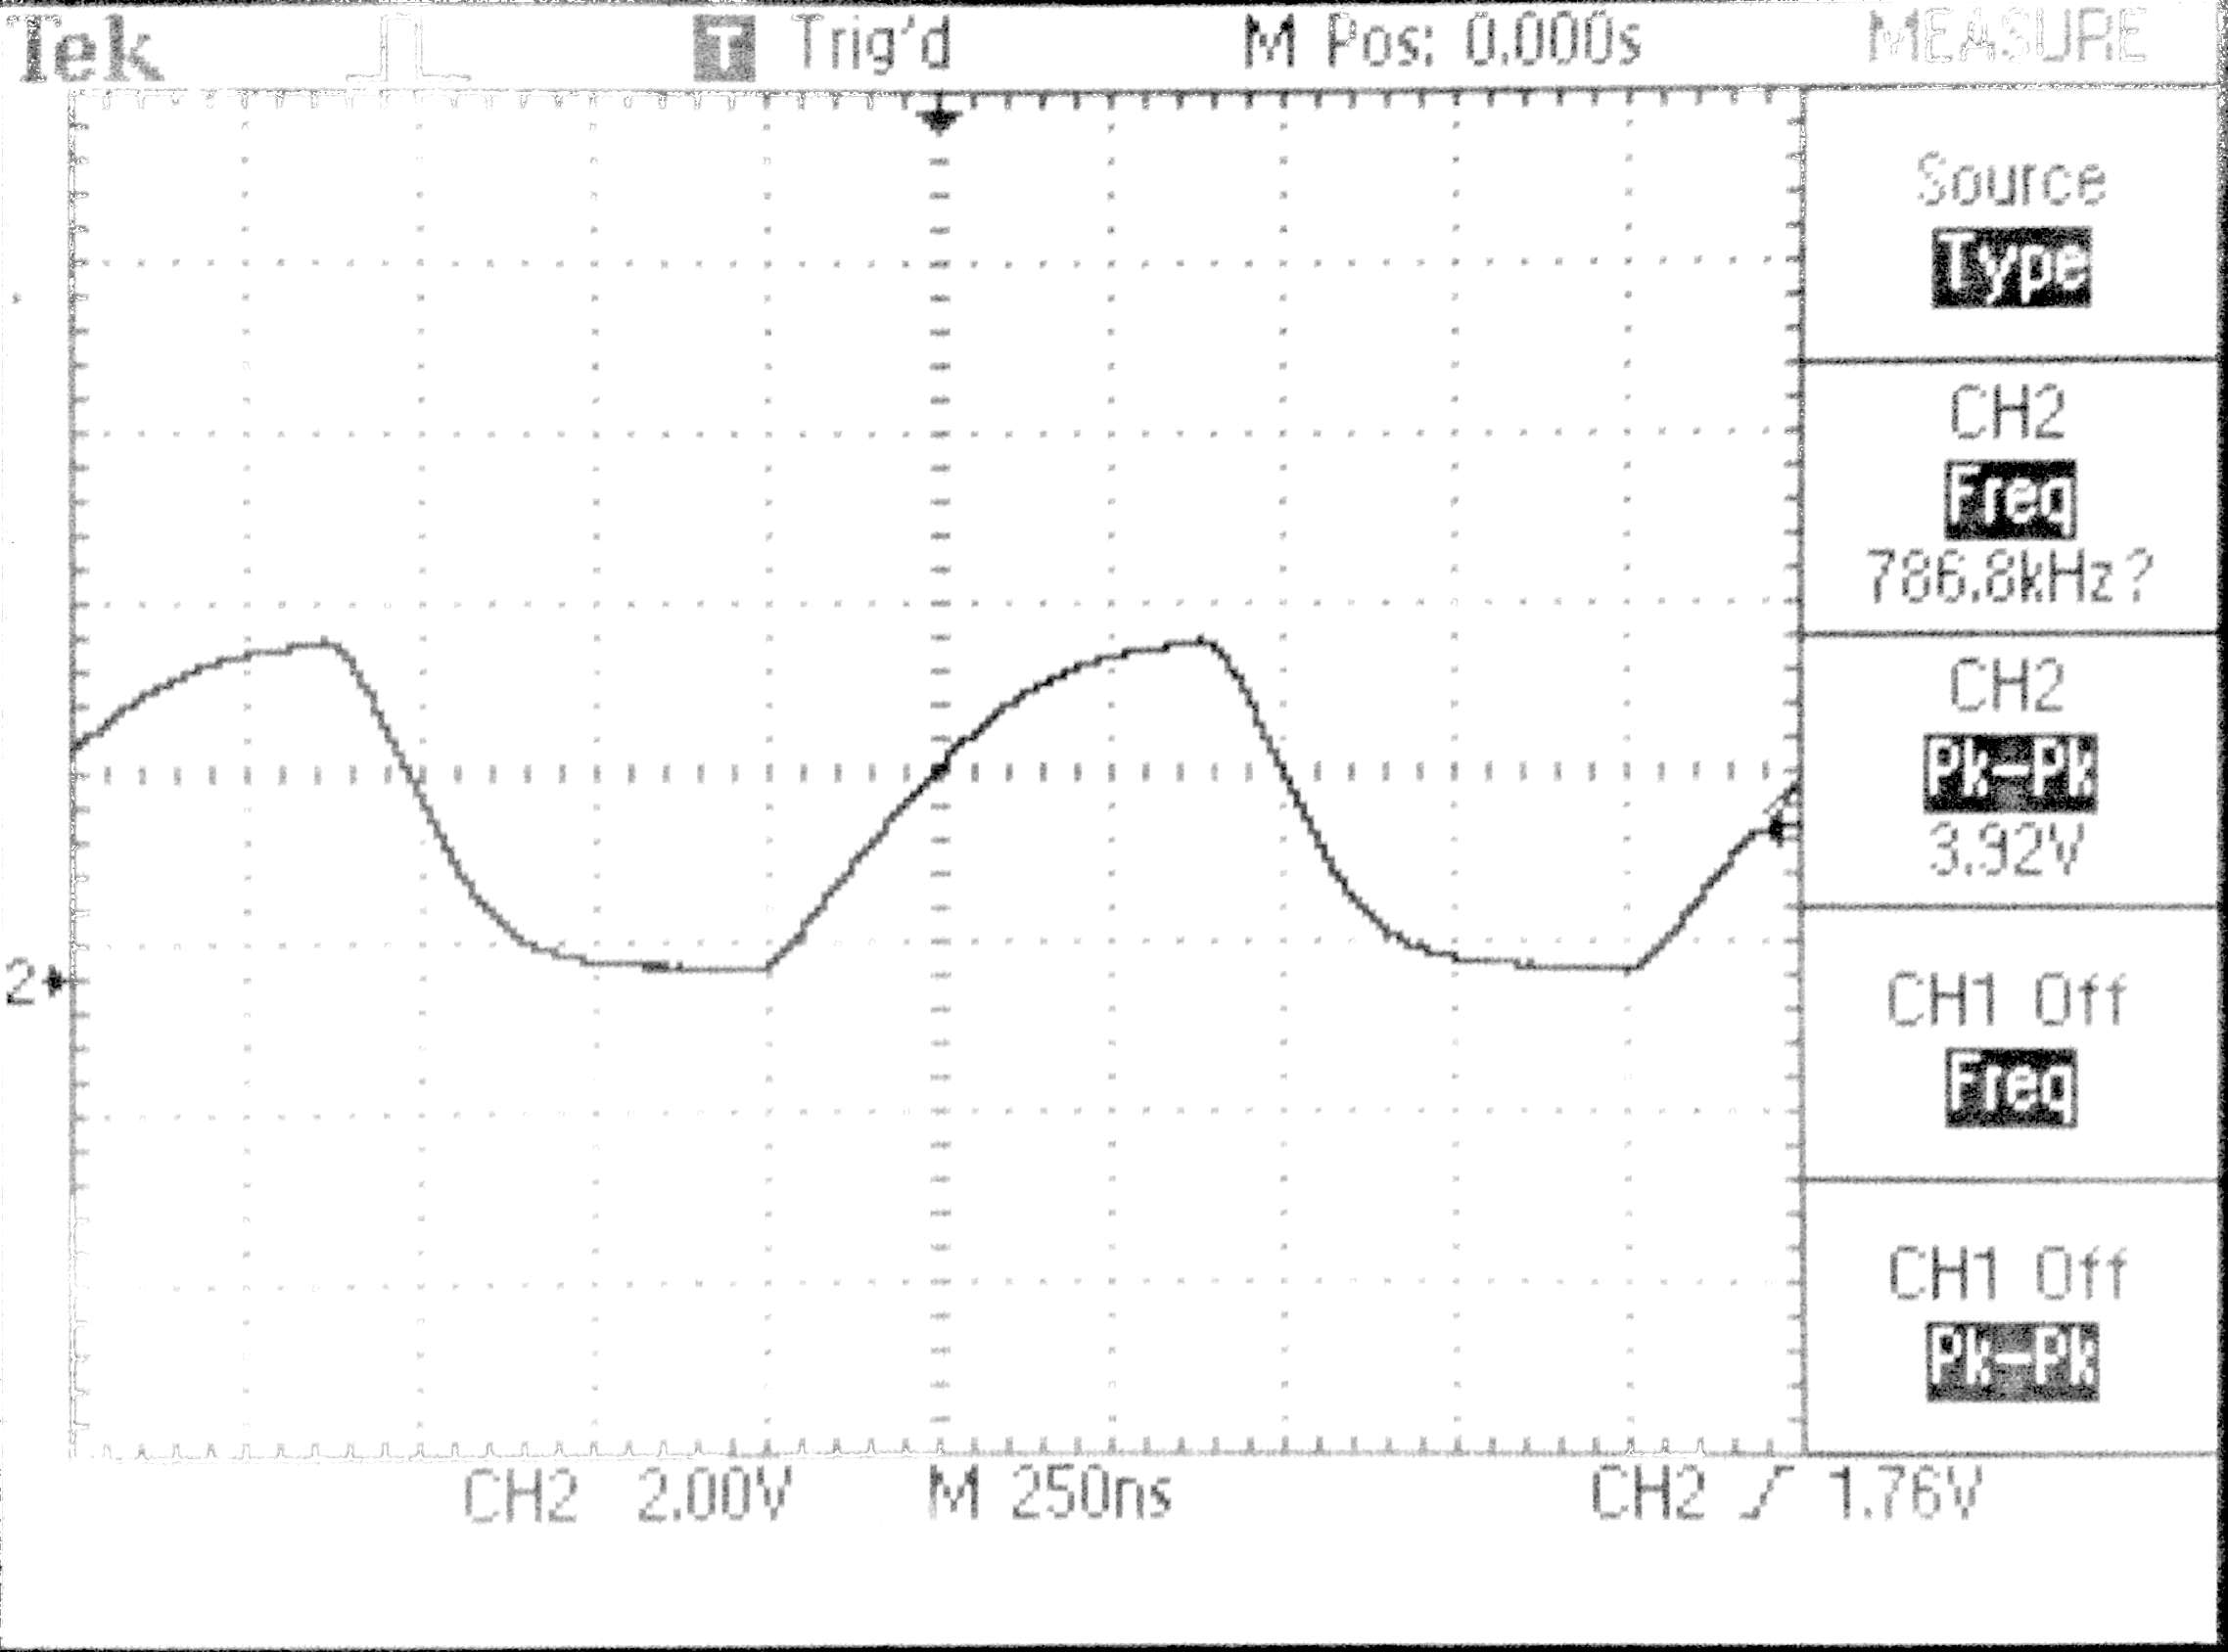
\includegraphics[width=2.5in]{EE214_5.jpg} \\
      \em V\textsubscript{DD} = 3 & \em V\textsubscript{DD} = 4 \\
         & \\
      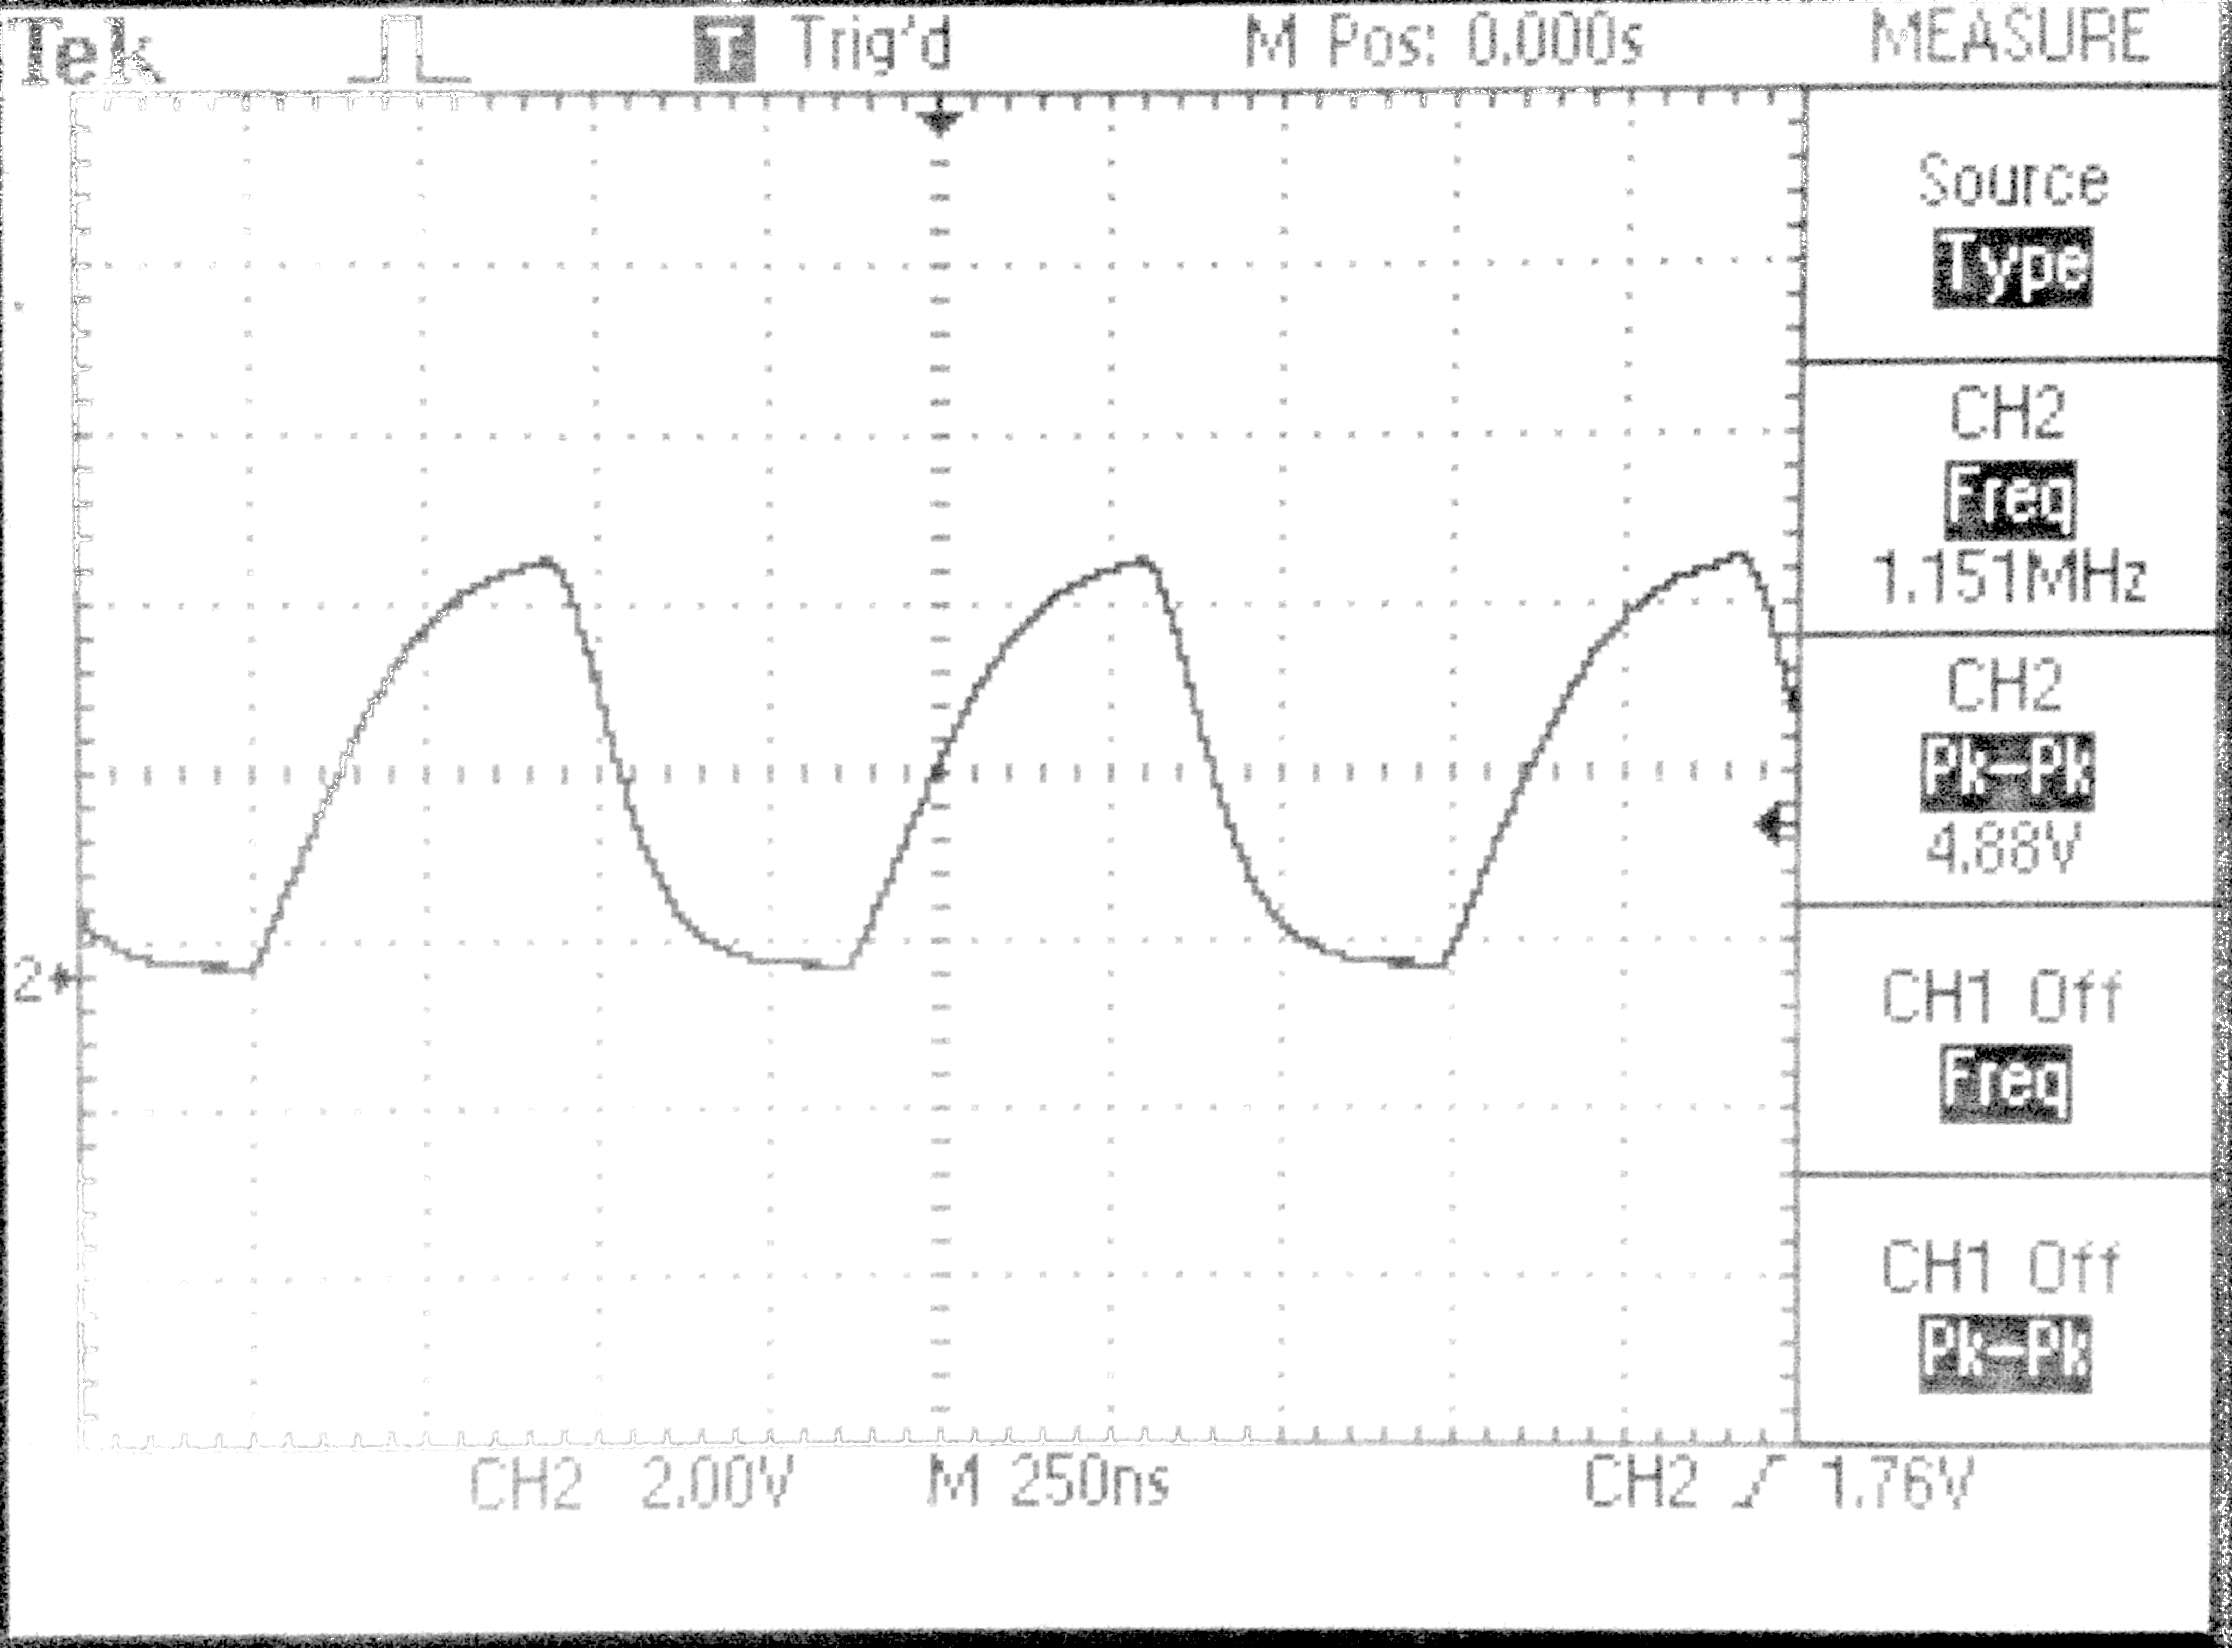
\includegraphics[width=2.5in]{EE214_1.jpg} & 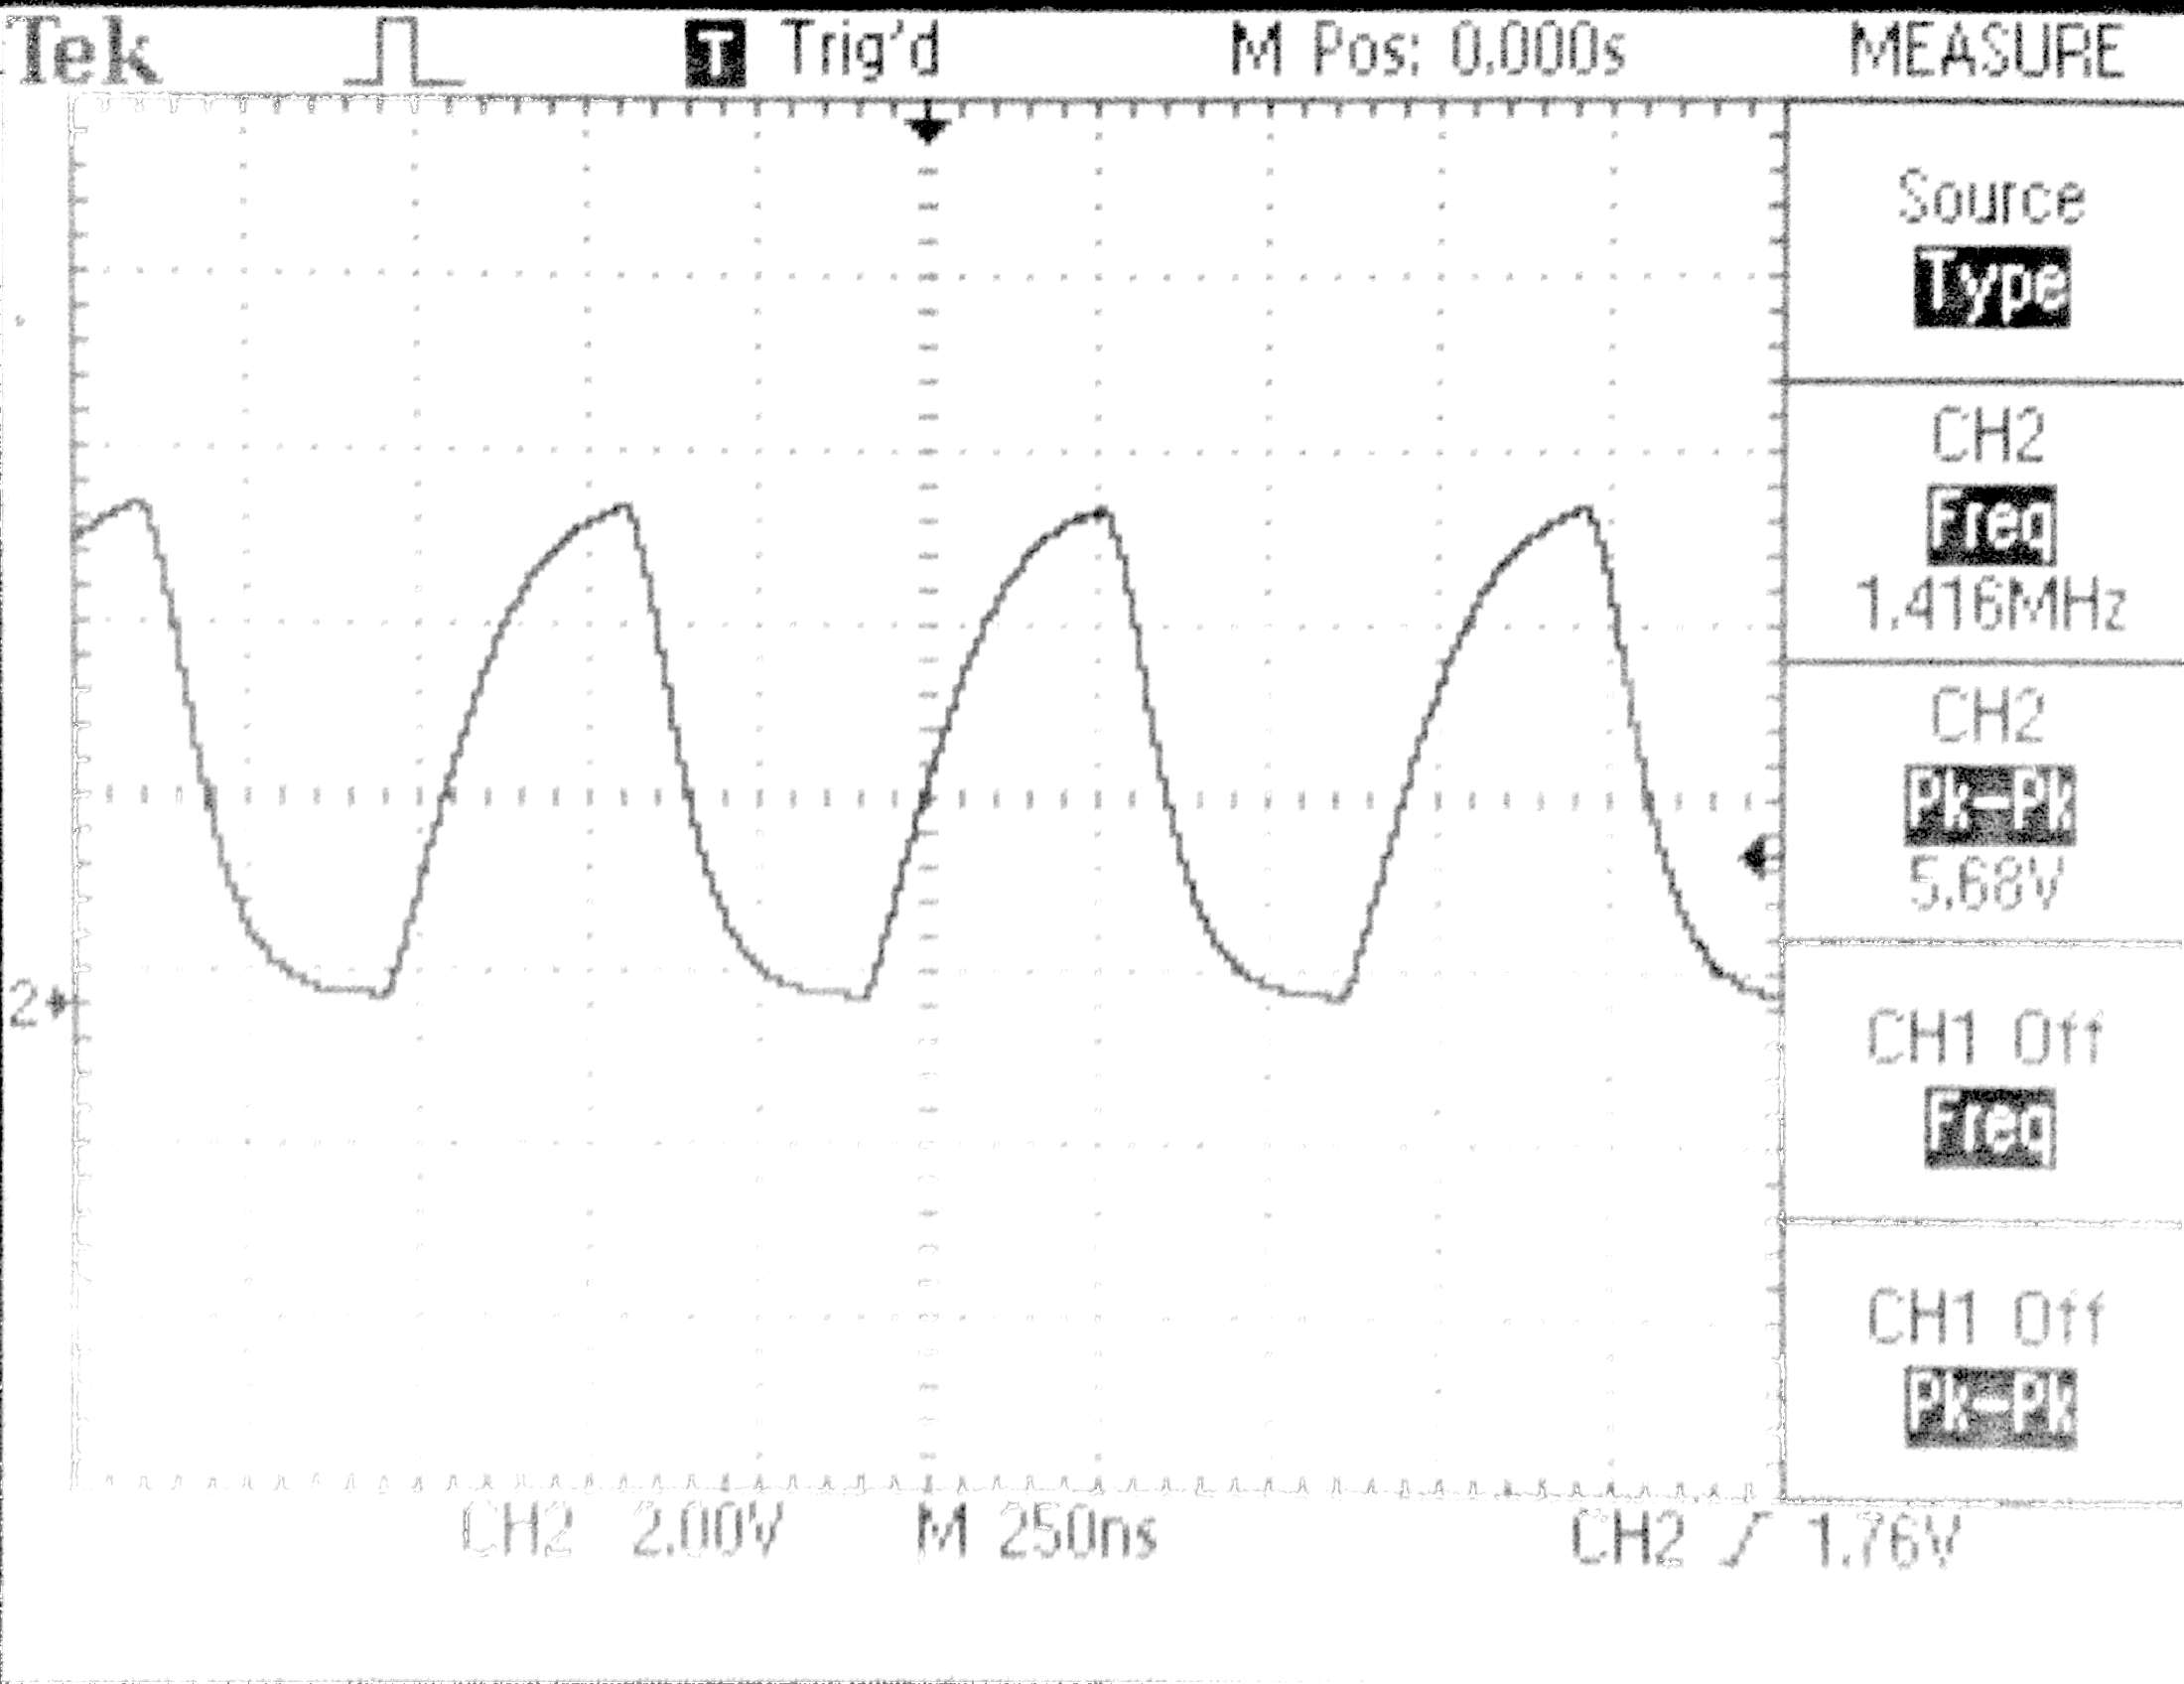
\includegraphics[width=2.5in]{EE214_6.jpg} \\
      \em V\textsubscript{DD} = 5 & \em V\textsubscript{DD} = 6 \\
  \end{tabular}
 \caption{Snapshots of the output waveform at different supply voltages {\em(Load = 2)}}
\end{table}

\begin{table}[H]
\centering
\begin{tabular}{| c | c |}
\hline
\bf Supply Voltage ($V_{DD}$) & \bf Frequency (MHz)\\
\hline
3 & 0.3922 \\
4 & 0.7868 \\
5 & 1.151 \\
6 & 1.416 \\
\hline
\end{tabular}
\caption{Variation of the frequency of oscillation with $V_{DD}$. {\em(Load = 2)}}
\end{table}

The reduction of the frequency with the increase in supply voltage is evident from the above snapshots, as suggested by the relation. This can be better represented as below. From the proportionality relation above, we expect the period of oscillation to go down inversely with the supply voltage. Figure 7 is in agreement with the formula, and hence the dependence can be verified.

\begin{figure}[H]
\centering
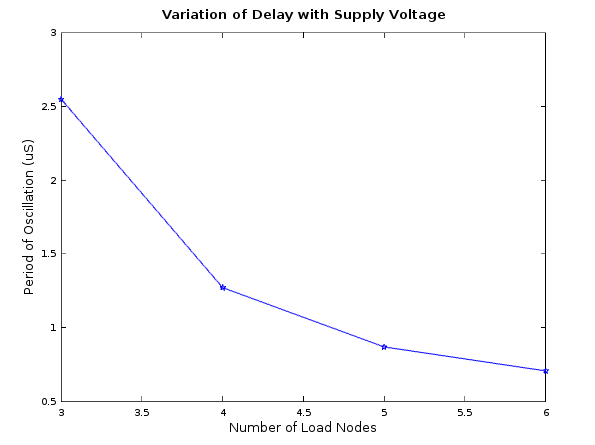
\includegraphics[scale=0.6]{Delay_Supply}
\caption{}
\end{figure}

\subsection{Current drawn by the Ring Oscillator}
Whenever an inverter output \emph{switches} from low to high, current is drawn from the power supply. The current drawn is approximately a triangular pulse whose width is essentially the delay of the gate. The current drawn by the ring oscillator is essentially the sum of the currents drawn by the individual inverters. \footnote{Note that, however, the switching events do not all happen at once. The signals do add, though.}\\
{\bf Measured Values:} \hspace{2em} $\langle I\rangle = -4.33mV $ \hspace{2em} $I_{P-P} = 22.4mV$
\begin{figure}[H]
\centering
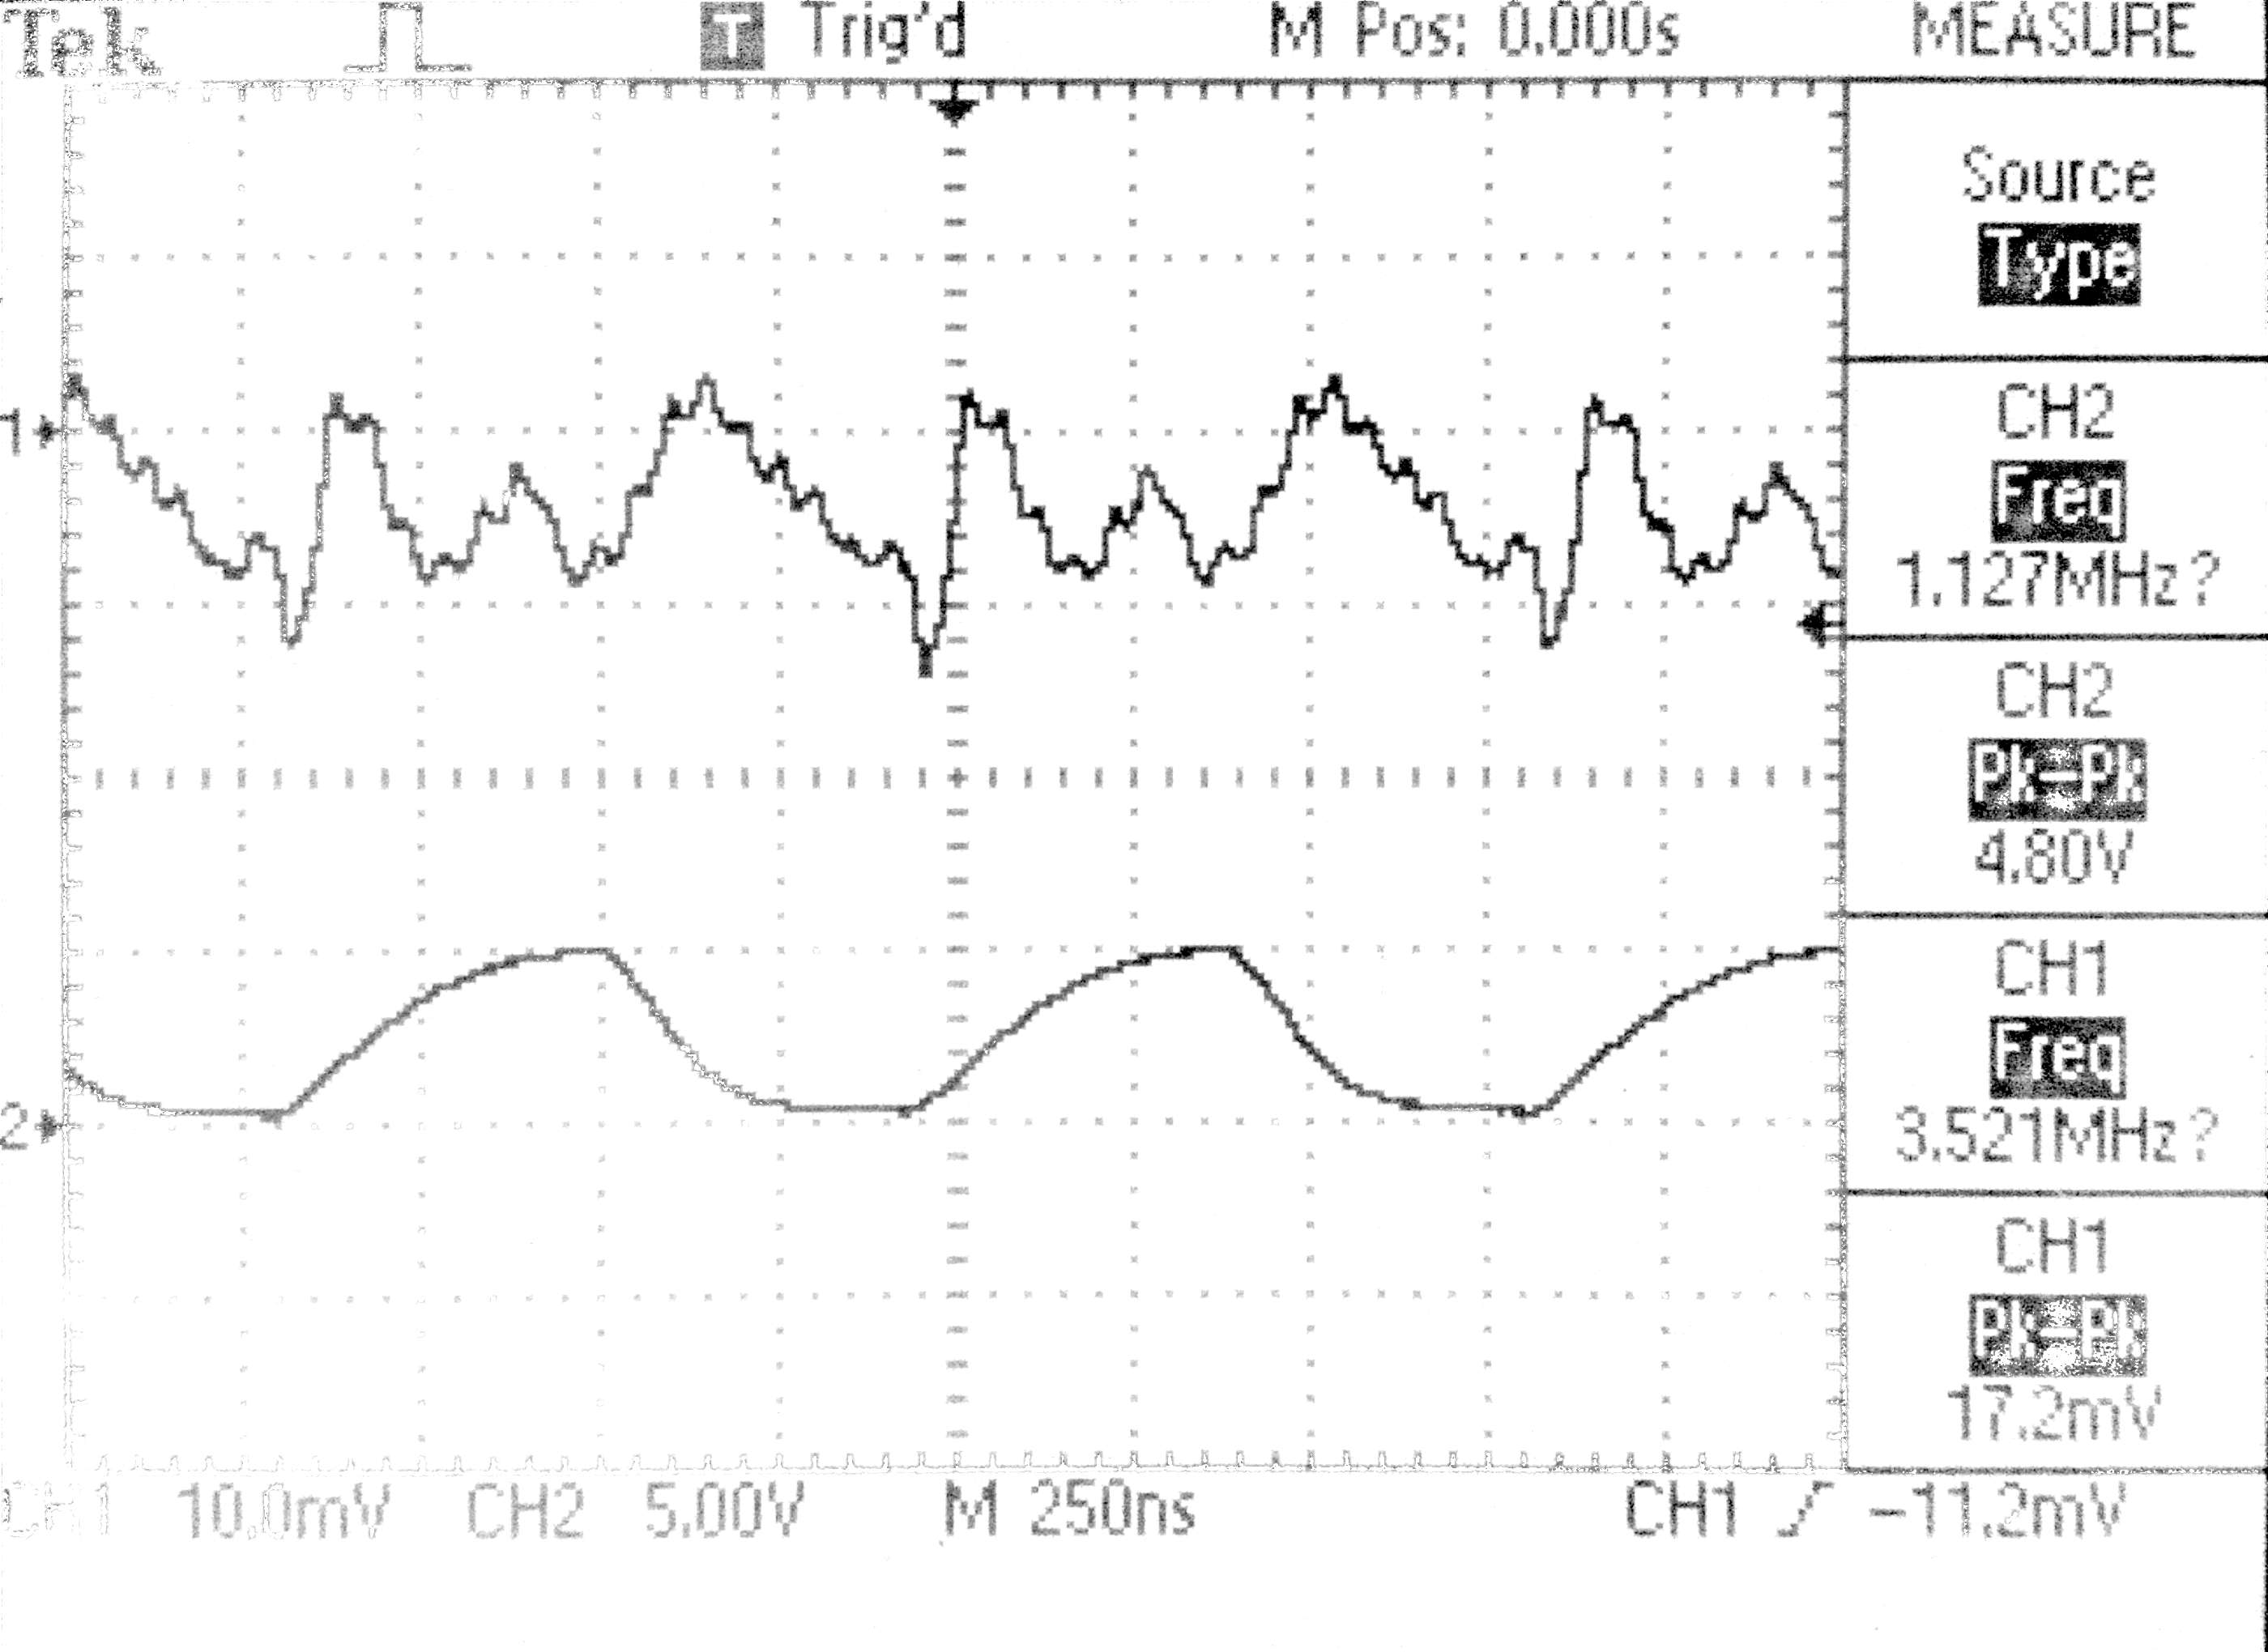
\includegraphics[scale=0.1]{EE214_8.jpg}
\caption{Snapshot of the DSO, measuring the switching current alongside $V_{out}$}
\end{figure}

\end{document}
